\documentclass[ASNA,twocolumn]{USG} %twocolumn
\usepackage{anyfontsize} %

\usepackage{colortbl}   % For coloring table lines
\usepackage{xcolor}     % For color definitions

\usepackage{pifont}     % checkmark/cross symbols used in comparison tables
\providecommand{\cmark}{\ding{51}}%
\providecommand{\xmark}{\ding{55}}%

\usepackage{steinmetz}
\graphicspath{{./images/}}
%\specialissue{}

\articletype{ORIGINAL ARTICLE}%
%\subarticletype{}

\received{20 January 2023}
\revised{21 January 2023}
\accepted{22 January 2023}
\journal{International Journal of Intelligent Systems}
\volume{0}
\copyyear{2026}
\startpage{1}
\articledoi{10.1002/0000}

%\raggedbottom

%%
%\renewcommand\ShowFrameLinethickness{0.15pt}
%\renewcommand*\ShowFrameColor{\color{red}}


\begin{document}
\title{An Adaptive, Closed-Loop CNN-LSTM Framework for Real-Time DoS/DDoS Detection and Mitigation in Software-Defined Networks under Concept Drift}
%\subtitle{Subtitle}
%\transtitle{}
%\subtranstitle{}
\author[1]{Tahir Ali}
\author[1]{Hasan Mahmood}
\author[2]{Muddasar Naeem}[https://orcid.org/0000-0003-0815-4883]
\author[3]{Asad Hussain}
\author[4]{Shumayla Yaqoob}
\author[2]{Antonio Coronato}[https://orcid.org/0000-0001-8177-032X]
\author[5]{Farman Ullah}




\authormark{ALI \textsc{et al.}}
\titlemark{Adaptive Closed-Loop CNN-LSTM for DDoS Detection and Mitigation in SDN}

\address[1]{\orgdiv{Department of Electronics }\orgname{Quaid-i-Azam University  }%
\orgaddress{\state{Islamabad, }\country{Pakistan}}}

\address[2]{\orgdiv{Artificial Intelligence and Robotics Lab, }\orgname{Università Giustino Fortunato, }%
\orgaddress{\state{Benevento, }\country{Italy}}}

\address[3]{\orgdiv{Department of Computer Science, University of  }\orgname{University of Reading, }%
\orgaddress{\state{Reading, }\country{UK}}}

\address[4]{\orgdiv{Faculty of Computing and Information Technology (FCIT) }\orgname{Sohar University, }%
\orgaddress{\state{Sohar, }\country{Oman}}}

\address[5]{\orgdiv{College of Information Technology (CIT) }\orgname{United Arab Emirates University, }%
\orgaddress{\state{Alain, }\country{UAE}}}

\corres{Farman Ullah  (\email{farman@uaeu.ac.ae}) }



%\fundingInfo{...}

\keywords{Software-defined networking | DDoS detection and mitigation | Concept drift | Online learning | Cross-dataset generalization | Hybrid CNN-LSTM}

%\transkeywords{}

\abstract[ABSTRACT]{Software-Defined Networking (SDN) centralizes control to make networks easier to operate, but the same centralization turns the controller into an attractive target for Denial-of-Service and Distributed Denial-of-Service (DoS/DDoS) attacks. Learning-based detectors for this problem have been proposed in large numbers, yet most share three weaknesses that limit their value in practice: they are trained once and then frozen, so accuracy decays when traffic shifts; they stop at raising an alert and never act on the network, so the claimed real-time benefit is never measured; and they are validated on the same dataset used for training, which says little about unseen traffic. This work treats those three issues as the problem to solve. We retain a compact CNN-LSTM model, in which the convolutional layers capture spatial structure in flow records and the recurrent layers model their temporal behavior, and build three capabilities around it. First, the detector adapts online: a drift detector monitors the live error rate and triggers short incremental updates, while a replay buffer preserves earlier knowledge and limits forgetting. Second, the detector runs in closed loop with the controller, installing OpenFlow rules to drop or rate-limit malicious sources so that the cost of mitigation can be measured rather than assumed. Third, the model is evaluated across datasets, trained on CICDDoS2019 and tested on the SDN-specific InSDN dataset and on live traffic from a Mininet, POX, and Open vSwitch testbed instrumented with sFlow. To keep the results trustworthy, class balancing is confined to the training folds and performance is reported on the natural class distribution using PR-AUC, the Matthews correlation coefficient, and per-class recall alongside accuracy. On CICDDoS2019 the model, with roughly 47,000 parameters, detects attacks at 99.95\% accuracy and an F1-score of 99.98\%; under simulated concept drift it recovers previously unseen attack families within about a dozen incremental updates, raising prequential accuracy from 0.59 to 0.93 where a static model stalls; and, trained on CICDDoS2019, it transfers to the SDN-specific InSDN dataset, where a brief adaptation step lifts zero-shot accuracy from 0.32 to 0.97. The detector also drives a closed-loop mitigation path on the controller within a Mininet, POX, and Open vSwitch testbed, measurably reducing Packet-In load on the controller; live per-source classification did not reliably distinguish the attacking hosts from the benign one in this testbed, and we report that finding alongside the mechanism it qualifies rather than omit it.
}


\abbr{AUC, area under the curve; CNN, convolutional neural network; DDoS, distributed denial-of-service; DL, deep learning; DoS, denial-of-service; FPR, false positive rate; LSTM, long short-term memory; MCC, Matthews correlation coefficient; ML, machine learning; OVS, Open vSwitch; ROC, receiver operating characteristic; SDN, software-defined networking; SMOTE, synthetic minority over-sampling technique.}

%\contributed{}

%\dedicated{}

\copyright{This is an open access article under the terms of the \href{Creative Commons Attribution-NonCommercial}{Creative Commons Attribution-NonCommercial} License, which permits use, distribution and reproduction in any medium, provided the
original~work~is~properly cited and is not used for commercial purposes.
\\[5pt]
  ©  2026 The Author(s). \textit{International Journal of Intelligent Systems} published by Wiley Periodicals LLC.}

%\openaccessstatement

\maketitle
%\afterpage{\aftergroup\restoregeometry}

%\onecolumn

\section{Introduction}\label{sec:introduction}
Software-Defined  Networking (SDN) is a major advancement in modern network architecture, which separates the control plane from the data plane \cite{singh2017survey}.This separation allows centralized network control, simplifying configuration, automation, and management. In this architecture as shown in Figure \ref{fig:sdnarchitecture}, the control plane decides how the traffic flows, while the data plane handles the actual forwarding of packets.  As a result, SDN has widespread adoption in data centers, enterprise environments, and cloud infrastructures where scalability and flexibility are in high demand. \cite{khorsandroo2021hybrid}.

Despite its benefits, the centralized architecture of SDN introduces significant security challenges. The SDN controller acts as the brain of the network \cite{paliwal2018controllers} and becomes a single point of failure for attackers \cite{eliyan2021and}. It is particularly vulnerable to DoS/DDoS attacks, which aim to exhaust system resources by flooding the controller with fake flow requests to disturb traffic volume \cite{de2023distributed}. The DoS attacks originate from a single source, and DDoS attacks harness large numbers of compromised devices across multiple locations, making them harder to detect and mitigate \cite{eliyan2021and}. These attacks compromise service availability, leading to network downtime, financial loss, and credibility damage. Such attacks are also often used to divert attention from more advanced breaches. The DDoS attacks are growing exponentially, both in frequency and sophistication. From early disruptions in 1999 and 2000, the scale of attacks has escalated dramatically, driven partly by the proliferation of Internet of Things (IoT) botnets \cite{gelgi2024systematic}. 
% These botnets exploit the widespread deployment of vulnerable, resource-constrained IoT devices, turning them into zombies (compromised devices) to launch large-scale, coordinated attacks. This evolution presents new challenges in advanced networking environments, particularly those leveraging SDN. The SDN architectures enable centralized traffic control and rapid response to network anomalies in order to target robust DDoS variants. 
%It also introduces critical vulnerabilities that high-volume and robust DDoS variants may target.%

Furthermore, emergence of low-rate, hard-to-detect attacks such as Shrew DDoS further complicates the detection efforts within SDN environments \cite{singh2023shrew}. The volume of IoT traffic continues to rise, and the AI detection mechanism is showing promise in detecting these sophisticated threats, making them a key focus in the development of resilient, SDN-aware security solutions \cite{bala2024ai}. The evolution of DDoS attacks over the past two decades reflects a significant increase in scale, automation, and technical sophistication as shown in Table \ref{tab:ddos_evolution}.These statistics highlight the growing complexity of modern threats in SDN environments.


\begin{table*}[htb!]
\centering
\caption{Evolution of Major DDoS Attacks and Emerging Threat Trends}
\label{tab:ddos_evolution}
\renewcommand{\arraystretch}{1.2}
\begin{tabular}{|p{1cm}|p{2.6cm}|p{3.5cm}|p{3.5cm}|p{3.5cm}|}
\hline
\textbf{Year} & \textbf{Incident or Campaign} & \textbf{Attack Characteristics} & \textbf{Target and Impact} & \textbf{Technical Significance} \\
\hline

2007 & Estonia Cyberattacks & Coordinated large-scale botnet-based DDoS & Government, banking, and media disruption & Early example of state-level cyber warfare \\
\hline

2012 & Operation Ababil & Sustained application-layer DDoS campaign & Major U.S. financial institutions & Prolonged financial-sector service disruption \\
\hline

2013 & Spamhaus DNS Amplification & Reflection/amplification attack (~300 Gbps) & Anti-spam organization infrastructure & Rise of DNS amplification techniques \\
\hline

2016 & Mirai Botnet Attack & IoT-driven volumetric DNS-targeted attack & Dyn DNS provider; global websites offline & Turning point toward IoT-based DDoS \\
\hline

2018 & GitHub Memcached Attack & 1.35 Tbps amplification attack & GitHub platform disruption & First terabit-scale DDoS attack \\
\hline

2020 & COVID-19 Era Surge & Increased reflection and multi-vector attacks & Cloud platforms and remote services & Expanded digital attack surface \\
\hline

2023 & HTTP/2 Hyper-Volumetric Attack & 201 million requests per second (RPS) & Global web infrastructure & Record-breaking application-layer DDoS \\
\hline

2024 & 3.45 Tbps Mega Attack & Multi-vector terabit-scale attack & Enterprises worldwide & Largest reported bandwidth-based DDoS \\
\hline

2025 & AI-Enhanced DDoS Campaigns & Adaptive botnets using automated traffic patterns & Cloud-native infrastructures & Emergence of AI-assisted attack strategies \\
\hline

2026 & IoT-Edge Distributed Attacks & Encrypted, ultra-distributed edge-based traffic & SDN/5G environments & Shift toward low-latency, encrypted attack vectors \\
\hline

\end{tabular}
\end{table*}



%%%%%%%%%%%%%%%%%%%%%%%%%%%%%% 
%%%%%%%%%%%%%%%%%%\subsection{Limitations of Existing Approaches}
 
The limitations of current DDoS detection approaches in SDN highlight the need for more robust solutions. Static rule-based systems use fixed rules and cannot adopt new attack patterns \cite{bringhenti2022automatic}. Traditional machine learning (ML) methods often suffer from high false positive rates (FPR) and lack real-time scalability \cite{ali2023machine}. Many ML models, such as random forest (RF), support vector machines (SVM), decision tree (DT), logistic regression (LR), naive bayes (NB), and k-Nearest neighbors (K-NN), are evaluated solely in simulated environments \cite{bansal2022comparative} or with outdated datasets \cite{gong2023survey}. These datasets often lack diversity and do not reflect the latest attack strategies or real-time traffic variations. These gaps emphasize the need for adaptive and lightweight solutions tested in real-world environments. 

%%%%%%%%%%%%%%%%%%%%%%%%%%%%%%%%%%%%%%%%%%%%%%
%%%%%%%%%%%%%%%%%%%%%%%%%%%%%%%%%%%%%%%
%%%%%%%%%%%%%%%%%\subsection{Motivation}

A large body of work already applies machine learning and deep learning to DDoS detection in SDN, and much of it reports near-perfect accuracy. Three weaknesses, however, keep recurring once these models are taken seriously as something to deploy. The first is that they are trained once, offline, and then left unchanged. When the traffic mix moves or a new attack variant appears, accuracy slips quietly until an operator notices and retrains the model by hand. The second is that the pipeline usually ends at the moment of classification. A model announces that an attack is in progress but does nothing to the network, so the real-time advantage that is so often claimed is never actually measured on the control plane. The third is evaluation: training and testing are drawn from the same dataset, which reveals little about how a detector copes with traffic it has not seen.

This paper is built around those three gaps rather than around the network architecture. We keep a compact CNN-LSTM model of roughly 47,000 parameters because it is inexpensive to run next to a controller and because its convolutional and recurrent halves are a natural fit for the spatial and temporal structure of flow records. The contribution is what we wrap around it: the model is allowed to adapt to drift while it runs, it is connected to a mitigation path inside the SDN control plane so that its decisions take effect, and it is tested on data that did not come from its training set.

% The architecture leverages the spatial pattern recognition strength of CNNs and the temporal sequence learning capability of LSTM networks. CNNs identify meaningful traffic characteristics such as packet size, variations, and flow durations, while LSTMs capture temporal behavior patterns that evolve. This synergy allows the model to detect both high-volume bursts and hard-to-detect slow-rate attacks, providing a robust and adaptive detection mechanism in dynamic SDN infrastructures.



%%%%%%%%%%%%%%%%%%%%%%%%%%%%%%%%%%%%%%%%%%%%%%%%%%%%%%%%%%%%
%%%%%%%%%%%%%%%%\subsection{Lightweight CNN-LSTM Architecture }

 %The proposed hybrid model is tailored for efficient and practical use in real-world environments. It uses eight carefully selected traffic features, significantly reducing the computational load and ensuring fast processing speeds suitable for real-time traffic monitoring. The compact architecture of the model consists of approximately 47,000 parameters that guide how the model makes decisions based on input data. This design achieves a balance between complexity and efficiency without compromising detection performance. Such a lightweight design ensures its feasibility for deployment in resource-constrained network environments and embedded SDN security systems.

%%%%%%%%%%%%%%%%Add title or no need? 
%%%%%%%%%%%%\subsection{Experimental Validation}

The evaluation is organized to test these three claims rather than a single accuracy number. The model is first trained on CICDDoS2019 \cite{cicddos2019dataset}, a benchmark that spans modern DDoS types across several protocols, including HTTP flood, UDP flood, TCP SYN flood, DNS amplification, and LDAP reflection. Generalization is then probed by testing the trained model on the SDN-specific InSDN dataset and on live captures from an emulated testbed, so that training and evaluation no longer come from the same source. The testbed itself uses Mininet with a POX controller, Open vSwitch for forwarding, and sFlow for traffic export, and it is where the closed-loop behavior is measured: on a positive detection the controller installs OpenFlow rules to drop or rate-limit the offending source. Concept drift is studied by presenting attack families as a stream and comparing a static model against the adaptive one. Throughout, class balancing with SMOTE and random undersampling \cite{ratnasari2024performance} is applied only inside the training folds to avoid leakage into the test set, and adaptive learning-rate scheduling and early stopping are used during training.

%%%%%%%%%%%%%%%%%%%%%%%%%%%%%%%%%%%%%%
%%%%%%\subsection{Performance Evaluation and Results}
On CICDDoS2019 the detector separates benign from malicious traffic with high accuracy at a low false positive rate, and reported on the natural class distribution rather than a rebalanced test set. More importantly for the argument of this paper, the adaptive variant recovers after drift where a frozen model loses accuracy, the model retains useful performance when moved to InSDN and to live testbed traffic, and the closed-loop defense reduces the controller's \texttt{Packet-In} load shortly after an attack begins while leaving legitimate flows largely undisturbed. Exact figures are reported in Section~\ref{sec:results_and_discussion}.


The main contributions of this work are as follows:
\begin{itemize}
    \item We make the detector adapt online. A drift detector watches the prediction error on the live stream and triggers short incremental updates to the CNN-LSTM model, while a replay buffer of earlier flows guards against catastrophic forgetting. This removes the manual-retraining assumption that underlies most prior SDN detectors and lets the model track changing traffic without being rebuilt from scratch.
    \item We close the loop between detection and the network. Once a source is flagged, the POX controller installs an OpenFlow rule to drop it, and we report the operational cost of doing so: controller load, the drop in \texttt{Packet-In} messages, and the classification-to-rule-install latency, on a real testbed rather than assumed. This turns the common ``real-time'' claim into measured behavior on the control plane; whether the mechanism reliably targets the attacker rather than legitimate traffic is a separate, open finding that we report rather than assume (Section~\ref{sec:threats}).
    \item We test generalization across datasets instead of within one. The model is trained on CICDDoS2019 and evaluated on the SDN-specific InSDN dataset and on live testbed captures, both with and without a brief adaptation step, which shows how well it transfers to traffic it was not trained on.
    \item We rebuild the evaluation protocol to remove flaws that inflate reported results. Class balancing is confined to the training folds, performance is reported on the natural (imbalanced) test distribution using PR-AUC, the Matthews correlation coefficient, and per-class recall in addition to accuracy, and the model is compared against deep-learning baselines re-implemented under identical splits with their parameter counts and inference latency reported.
\end{itemize}



The rest of the paper is organized as follows Section II Related work. Section III shows the proposed CNN-LSTM model, the description of the dataset, features selection, and training approach. The experimental set up and SDN testbed structure are described in Section IV. Section V is a discussion on the results and performance evaluation. Finally, Section VI provides the conclusion. 

\begin{figure*}[htb!]
\centering
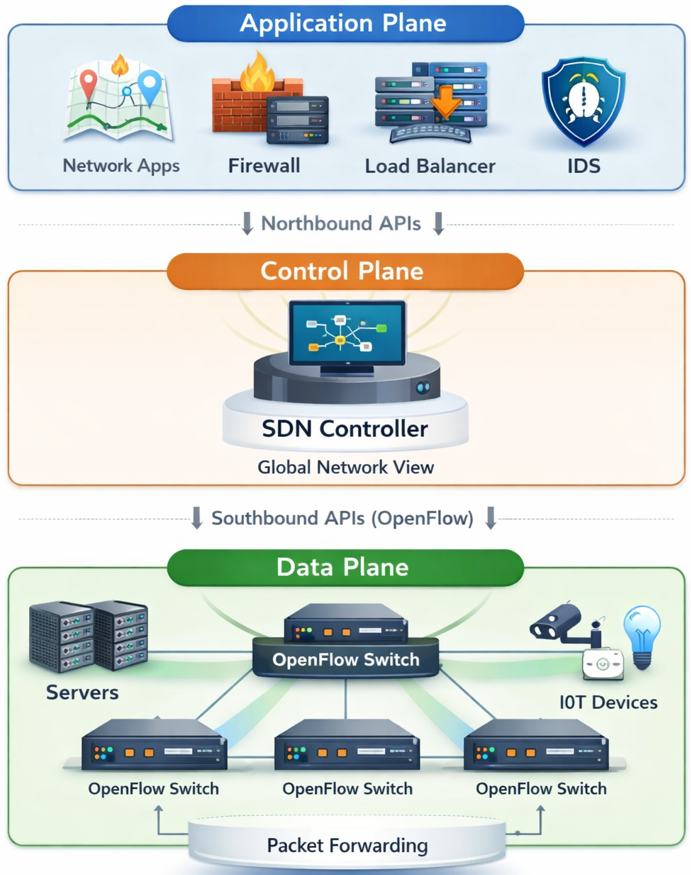
\includegraphics[width=0.95\textwidth]{sdnarchitecture.png}
\caption{Basic architecture of Software-Defined Networking (SDN), illustrating the separation of the application plane, control plane, and data plane with northbound and southbound communication interfaces.}
\label{fig:sdnarchitecture}
\end{figure*}


\section{Related Work}
\label{sec:related_work}
Over the past decade, the landscape of Internet-connected devices and cloud-based infrastructure has contributed to a significant rise in Distributed Denial-of-Service (DDoS) attacks. These attacks pose severe threats to SDN environments. The centralized control and programmability of SDN offer enhanced flexibility and scalability, but also introduce vulnerabilities \cite{alahmadi2023ddos}. In response, seekers have explored a wide range of detection techniques, ranging from traditional ML models to advanced DL and hybrid architectures,  to effectively overcome these threats. Despite substantial progress, key challenges remain in achieving real-time detection, lightweight deployment, and robust generalization across diverse traffic patterns. This related work presents a structured explanation of DDoS detection strategies in SDN, organized into traditional ML-based models, DL approaches, and hybrid frameworks \cite{jain2024comprehensive,dougan2025detection}. This organization provides clarity and reveals the landscape of networking, guiding seekers toward understanding both the strengths and limitations of existing approaches in literature while setting the stage for the proposed lightweight and high-performance solution proposed in the work.
%%%%%%%%%%%%%%%%%%%%%%%%%%%%%%%%%%%%%%%%%%%%%%%%%%%%%%%%%%%%%%%%%%%%%%%%%%%%
\subsection{Conventional Rule-Based Techniques for DDoS Detection}

Since the conventional DDoS detection techniques in SDN environments historically rely on straightforward mechanisms, such as signature-based filtering, threshold-based monitoring, and static rule application \cite{anand2024securing}. These approaches gained popularity due to their low computational tasks and ease of implementation. However, their effectiveness is often constrained to known attack patterns and static network behavior, making them inadequate in the face of evolving and dynamic threats.

Signature-based and rule-driven systems are employed in \cite{bhayo2021time, anand2024securing, fan2021detection}, which demonstrate a reasonable success against well-documented attacks. In these methods, predefined rules (signatures) based on traffic volume, frequency, and packet header patterns are used to identify malicious flows. While they are effective in static environments, these systems may easily be damaged \cite{maleh2023comprehensive} and fail to adapt to new or hidden attack vectors, especially those crafted to bypass static detection logic. However, attackers can manipulate packet attributes or distribute attack loads across multiple sources to avoid detection by such simplistic rules \cite{eliyan2021and}.

Threshold-based anomaly detection, as discussed in \cite{ma2023real}, presents a marginal improvement by identifying traffic patterns that exceed the defined limits. However, the rigidity of fixed thresholds leads to poor performance in fluctuating traffic conditions, a common characteristic of SDN networks, particularly in cloud and IoT-integrated infrastructures. The inability to dynamically recalibrate thresholds causes a surge in false positives during legitimate traffic spikes and delays detection during low-and-slow attack patterns. Another drawback of these traditional approaches is their lack of scalability. As SDN environments grow in size and complexity, the volume of traffic and control plane interactions increases significantly. Static mechanisms struggle to cope with such a scale without introducing latency or degrading detection accuracy. These methods lack the contextual awareness to detect multi-vector or robust attacks that evolve or utilize varying protocols, ports, and payloads to blend with normal traffic.

In essence, while traditional detection techniques laid the groundwork for securing SDN, their limitations in adaptability, scalability, and accuracy make them insufficient against modern DDoS threats \cite{hirsi2025comprehensive}. These shortcomings have paved the way for the integration of ML and intelligent systems that can learn from data, adapt to new behaviors, and offer real-time protection with higher precision.

 \subsection{Classical ML Techniques for DDoS Detection}

In order to address the inflexibility and limited generalization of traditional detection methods, researchers began incorporating classical ML algorithms for DDoS detection in SDN environments. In \cite{bansal2022comparative}, the DT, RF, SVM, LR, NB, and k-NN are offered the advantage of learning patterns from historical traffic data, allowing for more adaptive and intelligent detection mechanisms.

The work in \cite{tan2020new} employed a hybrid of K-Means clustering and DT to identify DDoS attacks, showing promising results on the NSL-KDD dataset. This combination enabled unsupervised clustering of traffic behaviors followed by supervised classification, while effective in academic settings \cite{lv2024hybrid}. The reliance of the model on the NSL-KDD dataset, a benchmark criticized for its age and lack of relevance to modern attack vectors, limits its real-world applicability. In \cite{khashab2021ddos}, the authors conducted a comparative analysis of multiple ML classifiers, including SVM, LR, NB, and k-NN. Although it highlighted the variability in performance across algorithms, the study lacked tailored feature engineering and lack to exploit SDN-specific attributes such as flow table dynamics or controller-switch interaction patterns.

In \cite{nadeem2022ddos}, researchers tested several classifiers such as RF, DT, SVM, and NB in a simulated SDN setup, showcasing decent accuracy levels. Yet, the simulations used simplified assumptions about attack traffic and did not fully replicate the complexity or volatility of live SDN deployments. Moreover, none of these methods accounted for latency or computational overhead in a real-time detection scenario—an essential consideration for SDN controllers operating under stringent performance constraints \cite{khashab2021ddos}. While models, such as RF and SVM, have proven robust across various domains, their effectiveness in DDoS detection heavily depends on the availability of high-quality labeled datasets. As demonstrated in \cite{hnamte2024enhancing} and \cite{xu2025deep}, many ML-based systems achieve high accuracy on curated datasets but perform poorly in production due to data drift, imbalanced class distributions, and unrecognized traffic behaviors \cite{palli2023combined}. Additionally, classical ML models generally lack temporal context, rendering them less effective in detecting robust or intermittent DDoS attacks that evolve.

A common limitation among these approaches is their static nature; models are often trained offline and require retraining to adapt to new attack signatures. This makes them less suitable for dynamic SDN environments, where rapid changes in topology and traffic behavior demand real-time adaptability \cite{alqahtani2024incremental}. While classical ML marked a significant improvement over static rule-based detection, it falls short in scalability, context-awareness, and continuous learning, setting the stage for more sophisticated DL and hybrid approaches.



\subsection{DL Techniques for DDoS Detection}

With the growing complexity of DDoS attacks and the dynamic nature of SDN traffic, classical ML approaches have shown significant limitations, particularly in their reliance on handcrafted features and lack of temporal modeling. The DL models have emerged as powerful alternatives, capable of automatically extracting hierarchical features and capturing temporal dependencies in network traffic. This has made DL particularly attractive for DDoS detection in SDN environments. Several studies \cite{nugraha2020deep, novaes2021adversarial, gadze2021investigation, priyadarshini2023sdn} have utilized CNN, LSTM, recurrent neural networks (RNNs),  and gated recurrent units (GRU) to model sequential traffic patterns and detect anomalies. For instance, the work in [3] implemented a hybrid CNN-LSTM architecture that achieved over 99\% accuracy in detecting slow DDoS attacks. The CNN layers extracted spatial features from traffic flows, while LSTM captured temporal relationships, making it effective for detecting long-duration and low-rate attacks that often evade classical methods.

In \cite{novaes2021adversarial}, the authors compared individual and hybrid DL models such as GAN, CNN, LSTM, and MLP, reporting high accuracy across multiple metrics, including precision and recall. GAN is particularly useful in generating adversarial samples for training, improving the robustness of detection. However, GAN-based approaches can be computationally intensive and may introduce instability during training. Studies such as \cite{gadze2021investigation} and \cite{priyadarshini2023sdn} incorporate attention mechanisms and Bidirectional (Bi) BiLSTM-CNN structures to further enhance performance. These models can dynamically focus on the most relevant parts of the input sequence, which improves detection in multi-vector attack scenarios. In \cite{priyadarshini2023sdn}, for instance, an attention-based BiLSTM-CNN model outperformed ten baseline methods across various datasets, indicating the strength of deep architectures in modeling complex attack behaviors.

Due to the strong performance of DL-based methods, they may face challenges. It often requires significant computational resources and large volumes of labeled training data, which may not always be available. Moreover, their black-box nature poses interpretability concerns for network administrators seeking transparency in decision-making. Many models \cite{shaheed2024hybrid, xu2025deep, min2023ddos} that report excellent performance on benchmark datasets, such as, CICDDoS2019 or CICIDS2017, may not generalize well in real-time deployments, particularly in edge computing scenarios with limited resources.

In summary, DL models offer substantial improvements in accuracy, flexibility, and temporal awareness over classical ML techniques. It is particularly well-suited for detecting sophisticated, evolving DDoS patterns in SDN environments. Nevertheless, their deployment must be balanced with considerations of computational cost, interpretability, and dataset diversity to ensure practical effectiveness. 

%%%%%%%%%%%%%%%%%%%%%%%%%%%%%%%%%%%%%%%%%%%%%%%%%%%%%%%%%%%%%%%%%%%%%%%%%%%%%%%%%%%%%%%%%%%%%%%%%%%%%%%%%%%%



% \begin{table*}[htb!]
% \centering
% \caption{Comparison of Existing DDoS Detection Models in SDN}
% \label{tab:comparison}
% \renewcommand{\arraystretch}{1.2}
% \begin{tabular}{|p{2.7cm}|p{4.2cm}|p{2.6cm}|p{2.4cm}|p{1cm}|p{1cm}|}
% \hline
% \textbf{Author and Reference} & \textbf{Model Type \& Techniques} & \textbf{Dataset Used} & \textbf{Accuracy / Metrics} & \textbf{Light- weight} & \textbf{Real-Time} \\
% \hline
% T. Liang et al.\cite{tan2020new} & K-Means + KNN (ML-based) & NSL-KDD & High (not quantified) & \xmark & \xmark \\
% \hline
% K. Fatima et al. \cite{khashab2021ddos} & LR, NB, KNN, SVM, DT, RF (ML) & Simulated TCP flood traffic & RF: 99.76\% & \xmark & \xmark \\
% \hline
% B. Nugraha \cite{nugraha2020deep} & CNN + LSTM (Hybrid DL) & Synthetic slow DDoS & Accuracy: >99\% & \xmark & \xmark \\
% \hline
% M. P. Novaes et al. \cite{novaes2021adversarial} & GAN, CNN, LSTM, MLP & CICDDoS2019 & GAN: 94.3\%, CNN: 94\% & \xmark & \xmark \\
% \hline
% M. W. Nadeem et al. \cite{nadeem2022ddos} & RF, SVM, KNN, DT (ML) & NSL-KDD & Not specified & \xmark & \xmark \\
% \hline
% A. Awais \cite{bhayo2021time} & SDNWISE-based Rule Matching & Simulated SDN Logs & No Accuracy Given & \cmark & \xmark \\
% \hline
% J.D. Gadze et al. \cite{gadze2021investigation} & SVM, Neural Networks & GitHub SDN-DoS Dataset & SVM: >95\% & \xmark & \xmark \\
% \hline
% H. Polat et al. \cite{polat2022novel} & LSTM, GRU, SVM (Hybrid TL) & Custom Traffic Data & 97.62\% & \xmark & \xmark \\
% \hline
% H. Elubeyd et al. \cite{elubeyd2023hybrid} & CNN + LSTM (Hybrid DL) & CICDDoS2019 & 99.81\%, 99.88\% & \xmark & \xmark \\
% \hline
% C. Fan et al. \cite{fan2021detection} & RF, DT, XGBoost, SVM (ML) & CICDDoS2019 & RF: 68.9\% & \xmark & \xmark \\
% \hline
% I. Priyadarshini et al. \cite{priyadarshini2023sdn} & Attention + Bi-LSTM-CNN & Kaggle DDoS Sets & 99.74\% & \xmark & \xmark \\

% \hline
% N.S. Jumaah et al. \cite{shaheed2024hybrid} & CNN + LSTM + Attention & CICDDoS2019 & 99.17\% & \xmark & \xmark \\
% \hline
% B. Habib et al. \cite{habib2024time} & CNN + LSTM & KDD Cup’99 & 99.82\% & \xmark & \xmark \\
% \hline
% Z. Xu et al. \cite{xu2025deep} & CNN + LSTM (Hybrid) & CICDDoS2019 & 99.67\% & \xmark & \xmark \\
% \hline
% N. U. Ain et al. \cite{ain2025securing} & RF + RFE + Edge Deployment & UNSW-NB15, BoT-IoT & 99\% & \cmark & \cmark \\
% \hline
% R. Ma et al. \cite{ma2023real} & RNN, LSTM, HTM, CNN (Ensemble) & CICDDoS2019 & 99.92\% & \xmark & \xmark \\
% \hline
% A.V. Songa et al. \cite{songa2024integrated} & CNN + LSTM + Autoencoder & CICDDoS2019 & 99.17\% & \xmark & \xmark \\
% \hline
% \rowcolor{gray!20}
% \textbf{T. Ali et al.} & \textbf{CNN + LSTM (Lightweight Hybrid using 8 Features)} & \textbf{CICDDoS2019 + Real SDN Testbed} & \textbf{Accuracy: 99.95\%}, \newline \textbf{Precision: 99.93\%}, \newline \textbf{Recall: 99.97\%}, \newline \textbf{FPR: 0.076\%} & \cmark & \cmark \\
% \hline
% \end{tabular}
% \end{table*}
 





\begin{table*}[htb!]
\centering
\caption{Comparison of DDoS Detection Models in SDN (Model-Level Analysis)}
\label{tab:comparison1a}
\renewcommand{\arraystretch}{1.2}
\begin{tabular}{|p{1.5cm}|p{1.5cm}|p{3.2cm}|p{2.2cm}|p{2.9cm}|p{2.9cm}|}
\hline
\textbf{Reference} & \textbf{Model Type} & \textbf{Used Model / Technique} & \textbf{Addressed Problem} & \textbf{Strength} & \textbf{Limitation} \\
\hline

\cite{tan2020new} & ML & K-Means + KNN & DDoS in SDN & Simple clustering-based detection & No real-time validation \\
\hline

\cite{khashab2021ddos} & ML & LR, NB, KNN, SVM, DT, RF & TCP Flood & High RF accuracy & Simulation-only dataset \\
\hline

\cite{nugraha2020deep} & Hybrid DL & CNN + LSTM & Slow DDoS & Captures spatial-temporal patterns & High computational cost \\
\hline

\cite{novaes2021adversarial} & DL & GAN, CNN, LSTM, MLP & Adversarial DDoS & Robust to adversarial traffic & Complex training \\
\hline

\cite{nadeem2022ddos} & ML & RF, SVM, KNN, DT & SDN DDoS & Comparative ML evaluation & Limited performance reporting \\
\hline

\cite{bhayo2021time} & Rule-based & SDNWISE Rule Matching & Flow rule attacks & Lightweight rule processing & No accuracy metric \\
\hline

\cite{gadze2021investigation} & ML & SVM, Neural Networks & SDN DoS & Strong classification capability & Dataset-dependent validation \\
\hline

\cite{polat2022novel} & Hybrid TL & LSTM, GRU, SVM & DDoS detection & Transfer learning integration & Limited scalability analysis \\
\hline

\cite{elubeyd2023hybrid} & Hybrid DL & CNN + LSTM & Large-scale DDoS & Very high accuracy & Heavy architecture \\
\hline

\cite{fan2021detection} & ML & RF, DT, XGBoost, SVM & Multi-vector DDoS & Ensemble comparison & Low RF performance \\
\hline

\cite{priyadarshini2023sdn} & DL & Attention + BiLSTM-CNN & SDN DDoS & Attention-enhanced learning & No deployment validation \\
\hline

\cite{shaheed2024hybrid} & Hybrid DL & CNN + LSTM + Attention & SDN DDoS & Multi-stage feature learning & Computational complexity \\
\hline

\cite{habib2024time} & Hybrid DL & CNN + LSTM & Time-aware DDoS & Strong temporal modeling & Uses older dataset \\
\hline

\cite{xu2025deep} & Hybrid DL & CNN + LSTM & SDN DDoS & High detection performance & Resource intensive \\
\hline

\cite{ain2025securing} & ML + Edge & RF + RFE & IoT/Edge DDoS & Lightweight + Edge-ready & Feature selection dependent \\
\hline

\cite{ma2023real} & Ensemble DL & RNN, LSTM, HTM, CNN & Real-time DDoS & Ensemble robustness & High complexity \\
\hline

\cite{songa2024integrated} & Hybrid DL & CNN + LSTM + AE & Integrated SDN security & Autoencoder integration & Not lightweight \\
\hline

\rowcolor{gray!20}
\textbf{Proposed Model} & \textbf{Lightweight Hybrid} & \textbf{CNN + LSTM (8 Features)} & \textbf{Real-time SDN DDoS} & \textbf{High accuracy + Efficient} & \textbf{Feature-reduction dependent} \\
\hline

\end{tabular}
\end{table*}   




\begin{table*}[htb!]
\centering
\caption{Dataset, Feature Engineering and Deployment Characteristics}
\label{tab:comparison1b}
\renewcommand{\arraystretch}{1.2}
\begin{tabular}{|p{2.2cm}|p{3.1cm}|p{3.5cm}|p{3.6cm}|p{1cm}|p{1cm}|}
\hline
\textbf{Reference} & \textbf{Dataset Used} & \textbf{Used Features} & \textbf{Preprocessing} & \textbf{Light- weight} & \textbf{Real-Time} \\
\hline

\cite{tan2020new} & NSL-KDD & KDD statistical features & Normalization & No & No\\
\hline

\cite{khashab2021ddos} & Simulated TCP traffic & Flow statistics & Feature scaling & No & No \\
\hline

\cite{nugraha2020deep} & Synthetic slow DDoS & Spatial-temporal features & Data reshaping & No& No\\
\hline

\cite{novaes2021adversarial} & CICDDoS2019 & Deep extracted features & Adversarial training & No & No \\
\hline

\cite{nadeem2022ddos} & NSL-KDD & KDD features & Feature selection & No & No\\
\hline

\cite{bhayo2021time} & Simulated SDN Logs & Flow-rule attributes & Rule matching & Yes  & No\\
\hline

\cite{gadze2021investigation} & GitHub SDN-DoS Dataset & Flow-based features & Normalization & No & No \\
\hline

\cite{polat2022novel} & Custom traffic data & Time-series features & Transfer learning prep. & No & No \\
\hline

\cite{elubeyd2023hybrid} & CICDDoS2019 & 70+ flow features & Standard scaling & No & No \\
\hline

\cite{fan2021detection} & CICDDoS2019 & Selected important features & Feature ranking & No & No \\
\hline

\cite{priyadarshini2023sdn} & Kaggle DDoS sets & Attention-weighted features & Data normalization & No & No \\
\hline

\cite{shaheed2024hybrid} & CICDDoS2019 & Hybrid spatial-temporal & Feature extraction & No & No\\
\hline

\cite{habib2024time} & KDD Cup’99 & KDD statistical features & Scaling & No & No \\
\hline

\cite{xu2025deep} & CICDDoS2019 & Flow + temporal features & Normalization & No & No \\
\hline

\cite{ain2025securing} & UNSW-NB15, BoT-IoT & Reduced subset (RFE) & Feature elimination & Yes & \cmark \\
\hline

\cite{ma2023real} & CICDDoS2019 & Ensemble-selected features & Aggregation & No & No\\
\hline

\cite{songa2024integrated} & CICDDoS2019 & Autoencoder-derived features & Dimensionality reduction & No & No\\
\hline

\rowcolor{gray!20}
\textbf{Proposed Model} & \textbf{CICDDoS2019 + SDN Testbed} & \textbf{8 Spatial-Temporal Features} & \textbf{Feature reduction + Normalization} & Yes & Yes  \\
\hline

\end{tabular}
\end{table*}
%%%%%%%%%%%%%%%%%%%%%%%%%%%%%%%%%%%%%%%%%%%%%%%%%%%%%%%%%%%%%%%%%%%%%%%%%%%%%%%%%%%%%%%%%%%%%%%%%%

\subsection{Hybrid Techniques for DDoS Detection}

Recognizing the individual limitations of standalone ML and DL techniques, recent research has increasingly turned toward hybrid models and multi-stage frameworks to enhance DDoS detection in SDN environments. These hybrid approaches aim to integrate the strengths of various models, such as the feature extraction capabilities of CNNs, the temporal learning of LSTM/GRU, and the interpretability of classical ML classifiers, to build more robust and adaptive solutions.

Numerous studies \cite{polat2022novel, elubeyd2023hybrid, habib2024time, xu2025deep, min2023ddos, nazir2024deep, ain2025securing, ma2023real, shaheed2024hybrid} explore these hybrid strategies with promising results. The work in \cite{elubeyd2023hybrid} proposed a hybrid DL model combining CNN and LSTM, which achieves accuracy above 99.8\% on the CICDDoS2019 dataset. By leveraging CNN for spatial pattern detection and LSTM for sequential learning, the model effectively captured volumetric and slow-rate attacks that often go undetected by simpler classifiers.

Other studies \cite{habib2024time, xu2025deep, min2023ddos} consider this further by incorporating attention mechanisms, dimensionality reduction techniques, and model optimization steps such as quantization and pruning. These enhancements not only improved accuracy but also reduced computational overhead, making such frameworks more suitable for real-time SDN deployments, including at the network edge.

More comprehensive systems, used in \cite{nazir2024deep} and \cite{ma2023real}, proposed multi-component pipelines. For instance, \cite{khaleel2023ddos} presented a layered model integrating LSTM, CNN, stacked autoencoders, and checkpoint networks to ensure fault tolerance and maintain detection integrity even in degraded conditions. Similarly, \cite{ma2023real} combined multiple tools, including recursive feature elimination (RFE), density-based spatial clustering of applications with noise (DBSCAN) clustering, (auto-regressive integrated moving average) is a statistical model for time series forecasting (ARIMA), and rule-based decision logic to build a resilient and interpretable anomaly detection system.

The hybrid models tend to offer improved detection performance and generalization capabilities, but they also introduce new challenges. The complexity of integrating diverse algorithms can lead to increased system overhead and difficulty in tuning hyperparameters. Furthermore, some solutions depend on customized datasets or controlled simulation environments, raising concerns about their generalization and reproducibility in real-world SDN networks \cite{bhayo2021time, nazir2024deep}.

Hybrid frameworks represent a pragmatic path forward, offering a balanced compromise between performance, robustness, and flexibility, particularly critical in SDN architectures that are inherently programmable and adaptive. As shown in \cite{ma2023real}, where an ensemble of RNN, LSTM, HTM, and CNN was employed, combining diverse neural architectures can significantly enhance the resilience and accuracy of detection systems across multiple datasets and traffic patterns. 

%%%%%%%%%%%%%%%%%%%%%%%%%%%%%%%%%%%%%%%%%%%%%%%%%%%%%%%%%


\subsection{Comparative Analysis of DDoS Detection Techniques}

The point of comparison here is not the headline accuracy alone. Almost every recent detector reports figures above 99\% on CICDDoS2019, so a single accuracy number no longer tells the methods apart and is a weak basis for claiming progress. Tables~\ref{tab:comparison1a} and \ref{tab:comparison1b} summarize the usual axes, model type, dataset, and reported metrics, and Table~\ref{tab:gap_matrix} adds the axes that actually distinguish a deployable system: whether the model keeps learning after deployment, whether it is built to cope with concept drift, whether detection is connected to a mitigation action, whether it is evaluated on data from outside its training set, and whether operational cost such as latency and controller overhead is reported at all.

Conventional ML models such as DT, RF, and SVM \cite{tan2020new, khashab2021ddos, nadeem2022ddos} perform well on static benchmarks like NSL-KDD but tend to degrade in the shifting traffic of an SDN and rarely report their deployment cost. Deep models \cite{priyadarshini2023sdn, hnamte2024enhancing, habib2024time, elubeyd2023hybrid, xu2025deep} reach high accuracy, yet they are trained once, evaluated within a single dataset, and stop at the moment of classification without acting on the network.

Table~\ref{tab:gap_matrix} makes the gap explicit. Across the surveyed work, online adaptation and explicit drift handling are almost entirely absent, closed-loop mitigation is uncommon, cross-dataset evaluation is rare, and the operational cost of running the detector is seldom quantified. The incremental IDS of \cite{alqahtani2024incremental} is a useful exception on the adaptation axis, and a few studies \cite{wang2024detection, hnamte2024ddos} couple detection with mitigation, but none of the surveyed methods address all of these concerns together.

We are deliberately cautious about the accuracy claim. The detection accuracy of the proposed model is competitive with the strongest hybrids rather than dramatically higher, and we do not claim to surpass the best reported figures on CICDDoS2019. The contribution is that comparable detection quality is delivered together with online adaptation, an instrumented mitigation loop, and cross-dataset evaluation, and at a stated computational cost. The supporting measurements are reported in Section~\ref{sec:results_and_discussion}.

\begin{table*}[hbt!]
\centering
\caption{Capability gap matrix: novelty axes addressed by prior work versus the proposed framework. \cmark{} = addressed, \xmark{} = not addressed.}
\label{tab:gap_matrix}
\renewcommand{\arraystretch}{1.2}
\begin{tabular}{|p{2.0cm}|c|c|c|c|c|}
\hline
\textbf{Reference} & \textbf{Online adaptation} & \textbf{Drift handling} & \textbf{Closed-loop mitigation} & \textbf{Cross-dataset eval.} & \textbf{Latency/ overhead reported} \\
\hline
\cite{tan2020new} & \xmark & \xmark & \xmark & \xmark & \xmark \\ \hline
\cite{khashab2021ddos} & \xmark & \xmark & \xmark & \xmark & \xmark \\ \hline
\cite{nugraha2020deep} & \xmark & \xmark & \xmark & \xmark & \xmark \\ \hline
\cite{novaes2021adversarial} & \xmark & \xmark & \xmark & \xmark & \xmark \\ \hline
\cite{elubeyd2023hybrid} & \xmark & \xmark & \xmark & \xmark & \xmark \\ \hline
\cite{priyadarshini2023sdn} & \xmark & \xmark & \xmark & \xmark & \xmark \\ \hline
\cite{xu2025deep} & \xmark & \xmark & \xmark & \xmark & \xmark \\ \hline
\cite{ma2023real} & \xmark & \xmark & \xmark & \xmark & \xmark \\ \hline
\cite{ain2025securing} & \xmark & \xmark & \xmark & \xmark & \cmark \\ \hline
\cite{wang2024detection} & \xmark & \xmark & \cmark & \xmark & \xmark \\ \hline
\cite{alqahtani2024incremental} & \cmark & \cmark & \xmark & \xmark & \xmark \\ \hline
\rowcolor{gray!20}
\textbf{Proposed} & \cmark & \cmark & \cmark & \cmark & \cmark \\ \hline
\end{tabular}
\end{table*}

%%%%%%%%%%%%%%%%%%%%%%%%%%%%%%%%%%%%%%%%%%%%%%%%%%%%%%%%%%%%%%%%%%%%%%%%%%%%%%%%%%%%%%%%%%%%%%%%%%%%%%%%%%%%%%%%%%

\section{Proposed Methodology} \label{sec:methodology}

This section explains the systematic approach adopted for designing, training, and validating the proposed model for DDoS detection in SDN environments. The methodology follows a structured process that includes data collection and preprocessing, hybrid model architecture, model training and validation, performance evaluation, and real-time testing in an SDN setup. Each of these steps ensures that the model is both effective and suitable for deployment in real environments, with a focus on scalability, efficiency, and high detection accuracy. 

%%%%%%%%%%%%%%%%%%%%%%
\subsection{Data Collection and Preprocessing}
The proposed model is trained using the CICDDoS2019 dataset \cite{cicddos2019dataset}, a contemporary benchmark that captures realistic DDoS attack scenarios across multiple protocols, including SYN, UDP, HTTP floods, and DNS amplification. The dataset offers a wide range of flow-based features representing traffic behavior essential for identifying both benign and malicious patterns.

Before preprocessing, an initial data analysis is performed to understand the distribution of traffic classes, detect anomalies, and identify relevant features. This step highlights the presence of significant class imbalance and redundancy in features. Based on this analysis, eight traffic features are carefully selected to reduce dimensionality while preserving key behavioral indicators for effective detection.

A structured preprocessing pipeline is then applied to prepare the data for DL. Column names are cleaned for consistency, and missing or infinite values are handled to eliminate distortions. Label values are standardized by mapping benign to 0 and malicious to 1, enabling binary classification.

Class imbalance can bias the model toward the dominant class, but it must be corrected without contaminating the evaluation. The order of operations therefore matters, and we deliberately split the data before any resampling. The dataset is first divided into training and testing partitions with stratified sampling, and only the training partition is balanced: synthetic minority over-sampling (SMOTE) together with random undersampling is applied inside the training folds alone, so that no synthetic or duplicated sample can reach the test set. The z-score standardization is fitted on the training data and then applied unchanged to the test data, again to keep test statistics out of training. The test set is left at its natural class ratio, which means that every metric we report reflects the imbalance a detector would actually meet in operation rather than an artificially balanced view. After scaling, the data are reshaped into the three-dimensional form (samples, timesteps, features) expected by the CNN-LSTM. Applying SMOTE before the split, as is common in the literature, leaks information across the partition boundary and inflates the reported scores; avoiding this is one of the corrections this work makes to the standard protocol.

Preprocessing is essential not just for cleaning the data but also for enhancing model performance. It ensures consistent feature scaling, balanced class distribution, and structured input format factors critical to achieving reliable convergence and robust detection accuracy. Without this stage, even a well-designed model may fail to learn meaningful patterns or generalize to real-world traffic.
%%%%%%%%%%%%%%%%%%%%%%%%%%%%%%%%%%%%%%%%%%%%%%%%%%%%%%%%%%%%%%%%%%%%%%%%%%%%%%%%%%%%%%%%%%%%%%%%%%%%%%%%%%%%%%%%%%%%%%%%%%%%%%%%%%%%%%%%%%%%%%%%%%%%%
\subsection{Feature Selection and Justification}


\begin{table*}[hbt!]
\centering
\caption{Selected Features and Justification for DDoS Detection in SDN}
\label{tab:feature_justification}
\begin{tabular}{|p{3cm}|p{4.5cm}|p{8cm}|}
\hline
\textbf{Feature} & \textbf{What it Measures} & \textbf{Why It Is Used Here} \\
\hline
Flow Duration & Total time a flow lasts & Long durations may indicate persistent attack flows such as Slowloris or low-rate DDoS \\
\hline
Fwd Packet Length Mean & Average size of forward packets & Helps identify anomalies in application-layer DDoS traffic patterns \\
\hline
Flow Packets/s & Packet transmission rate & High packet rates are common in volumetric DDoS attacks \\
\hline
Bwd Packet Length Mean & Average size of backward packets & Reflects client-server response imbalance typical in flooding \\
\hline
Fwd Header Length & Total header size of forward packets & Abnormal header sizes may signal spoofing or crafted attack packets \\
\hline
ACK Flag Count & Number of ACK flags & High ACK counts may indicate TCP ACK flooding \\
\hline
Init\_Win\_bytes\_forward & Initial TCP window size & Detects abnormal TCP configuration used in volumetric attacks \\
\hline
min\_seg\_size\_forward & Minimum segment size & Irregular segment size helps detect slow or probing attacks \\
\hline
\end{tabular}
\end{table*}



Feature selection is an essential part in designing efficient and accurate DDoS detection systems \cite{chanu2023dynamic}, especially in SDN environments. Many features are irrelevant or redundant in high-dimensional traffic datasets, which can degrade the performance of ML/DL models \cite{rane2024machine}. By selecting discriminative features, we reduce computational complexity, avoid overfitting, and improve generalization. Moreover, SDN environments require real-time response to network threats \cite{de2020near}. Therefore, effective and lightweight feature sets enhance both scalability and deployment feasibility.

The proposed model is trained and contains over 85 traffic features generated via CICFlowMeter \cite{ali2022ddos}. These features are extracted from flow-level metadata, similar to NetFlow-style records, which summarize network communications using packet header information. From this large dataset, we selected eight key features based on a combination of domain knowledge, correlation analysis, and exploratory data analysis (EDA). These features are primarily drawn from the network (Layer~3) and transport (Layer~4) layers of the OSI model and capture essential aspects of traffic behavior such as session duration, packet sizes, and transmission rates.

Several selected features (Figure \ref{fig:feature_dists}), such as \texttt{ACK Flag Count} and \texttt{Init\_Win\_bytes\_forward}, are specific to the TCP protocol and provide insight into connection-level behaviors. Others, such as \texttt{Flow Duration} and \texttt{Flow Packets/s}, are protocol-agnostic and reflect general flow characteristics. This combination allows our model to detect both volumetric and complex DDoS attacks across different protocol types. The selected features are summarized in Table \ref{tab:feature_justification}.

% The correlation heatmaps and distribution plots, as shown in Figure \ref{fig:corr_heatmap}  and Figure \ref{fig:feature_dists}, are generated during EDA to validate the chosen features. The correlation matrix (Figure \ref{fig:corr_heatmap}) demonstrates minimal redundancy among the selected features, with most pairwise Pearson correlation values below 0.5. This ensures each feature contributes unique information. Additionally, feature distribution plots (Figure \ref{fig:feature_dists}) show structured but skewed distributions typical in network traffic data, confirming that these features capture realistic variability between benign and malicious traffic.

% \begin{figure*}[hbt!]
% \centering
% \includegraphics[width=\textwidth, height=0.6\textheight]{heatmap.png}
% \caption{Correlation Heatmap of Selected Features}
% \label{fig:corr_heatmap}
% \end{figure*}


\begin{figure*}[hbt!]
\centering
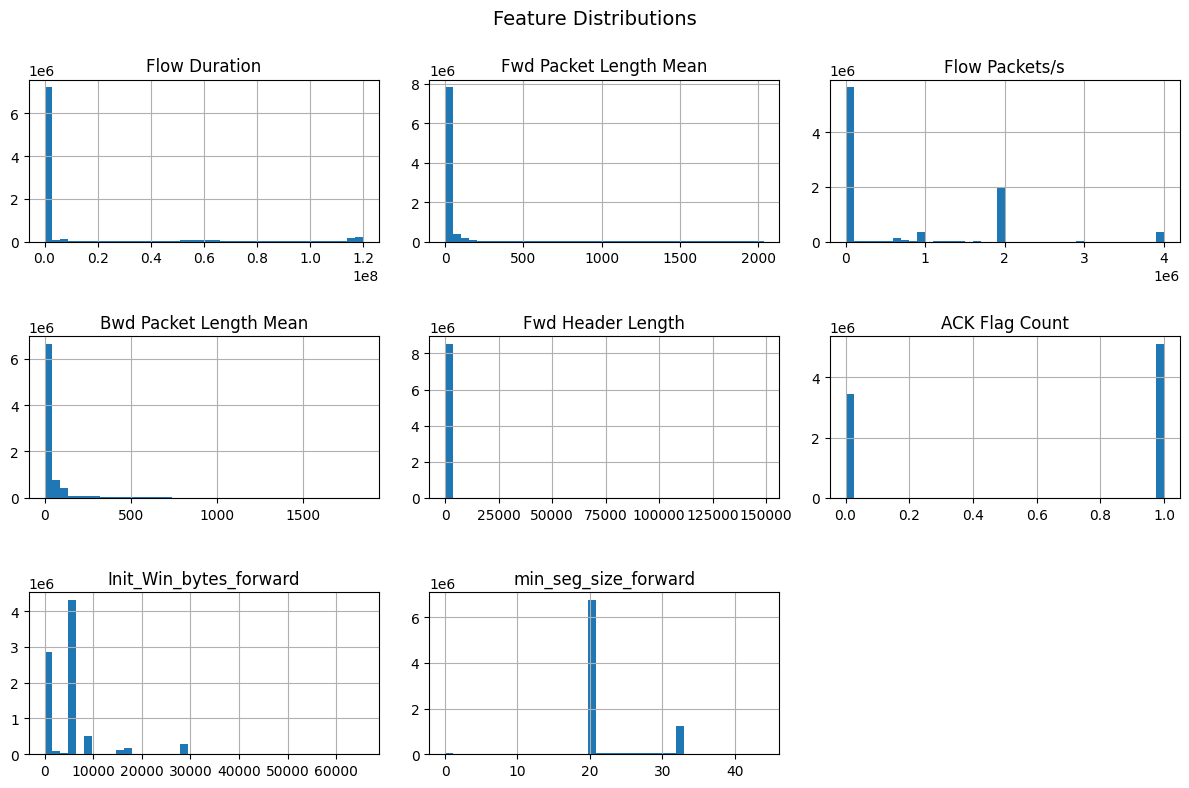
\includegraphics[width=\textwidth, height=0.6\textheight]{Featuredistribution.png}
\caption{Distribution Plots of Selected Features}
\label{fig:feature_dists}
\end{figure*}


We used the Pearson correlation coefficient for feature relevance to measure the linear dependence between pairs of features. The coefficient is computed using the following formula:

\begin{equation}
r_{XY} = \frac{\sum_{i=1}^{n}(X_i - \bar{X})(Y_i - \bar{Y})}{\sqrt{\sum_{i=1}^{n}(X_i - \bar{X})^2 \sum_{i=1}^{n}(Y_i - \bar{Y})^2}}
\label{eq:pearson}
\end{equation}

In this equation, $r_{XY}$ denotes the Pearson correlation coefficient between two variables $X$ and $Y$; $X_i$ and $Y_i$ represent the individual values of $X$ and $Y$ at the $i$-th observation; $\bar{X}$ and $\bar{Y}$ are the respective means of $X$ and $Y$; and $n$ is the total number of observations. This expression is the centered (mean-subtracted) form of the Pearson product-moment correlation coefficient, which is algebraically equivalent to the raw-score version commonly found in statistical literature \cite{mei2022modeling}. The coefficient $r_{XY}$ ranges from $-1$ to $1$, indicating the strength and direction of the linear relationship between the two variables. A value of $r_{XY}$ close to $0$ suggests a weak or no linear correlation, whereas values near $-1$ or $1$ indicate strong negative or positive linear correlation, respectively. In our analysis, features exhibiting a high degree of correlation (i.e., $|r_{XY}| > 0.9$) are considered redundant and subsequently excluded from further processing \cite{ma2023ddos}.


We also applied information-theoretic measures \cite{alalhareth2023improved}, such as information gain, to assess the discriminative power of each feature. The information gain (IG) between a feature $X$ and the target variable $Y$ is defined as:

\begin{equation}
IG(Y\mid X) = H(Y) - H(Y\mid X)
\label{eq:infogain}
\end{equation}

Here, $IG(Y\mid X)$ denotes the information gain obtain about the target variable $Y$ given knowledge of the feature $X$; $H(Y)$ represents the entropy of $Y$, and $H(Y\mid X)$ is the conditional entropy of $Y$ given $X$. Entropy $H(Y)$ quantifies the uncertainty or unpredictability in $Y$ and is defined as:

\begin{equation}
H(Y) = - \sum_{y\in{Y}} p(y) \log p(y)
\label{eq:entropy}
\end{equation}

In this equation, $Y$ is the set of possible outcomes of $y$, and $p(y)$ is the probability of outcome $y$. The conditional entropy $H(Y \mid X)$ similarly measures the expected uncertainty in $Y$ after observing $X$. Information gain thus captures the reduction in uncertainty about the target variable when a given feature is known. Higher values indicate more informative features. This analysis helped identify features that maximally reduced class uncertainty. The correlation and entropy-based assessments ensured that the selected features are independent and informative, ideal for training deep learning models.

%%%%%%%%%%%%%%%%%%%%%%%%%%%%%%%%%%%%%%%%%%%%%%%%%%

Prior studies have also validated the effectiveness of these features in identifying various DDoS variants, including volumetric, protocol abuse, and slow-rate attacks, particularly in SDN environments.

%%%%%%%%%%%%%%%%%%%%%%%%%%%%%%%%%%%%%%%%%%%%%%%%%%%%%%%%%%%%%%%%%%%%%%%%%%%%%%%%%%%%%%%%%%%%%%%%%%%%%%%%%%%%%%%%%%%%%%%%%%%%%%%%%%%%%%%%%%%%%%%%%%%%%%%%%%%%%%%%%%%%%%%%%%%%%%%%%%%%%%%%%%%%%%%%%%%%%%%%%%%%

\subsection{Attack Flow and Detection Strategy}

SDN introduces a logically centralized control plane, which makes it highly flexible but also vulnerable to DoS/DDoS attacks \cite{wang2024detection}. In such attacks, adversaries flood the OpenFlow switch with a high volume of new flow requests. Each of these requests triggers a \texttt{Packet-In} message to the SDN controller, eventually leading to excessive control plane load, flow table flood, and controller resource exhaustion.

\begin{figure*}[hbt!]
\centering
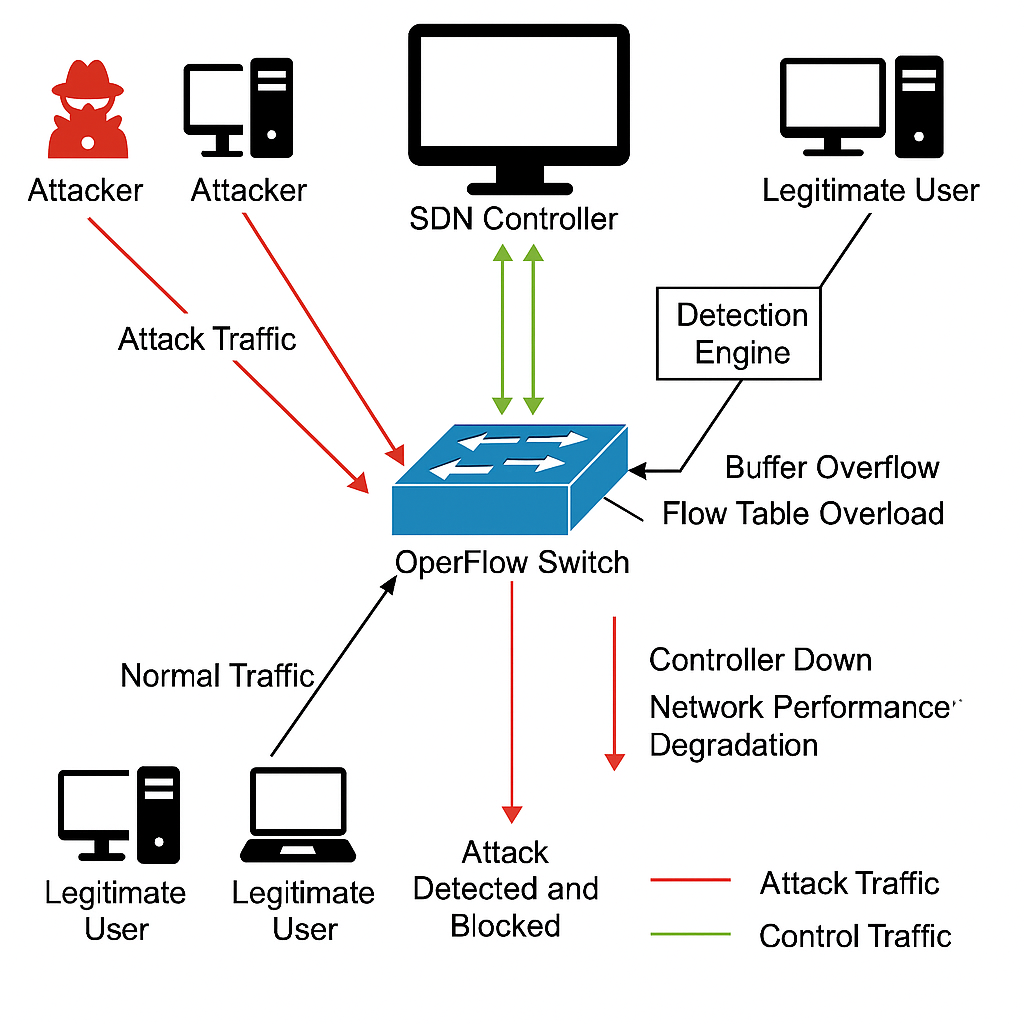
\includegraphics[width=0.7\textwidth, height=0.4\textheight]{attack_flow_diagram.png}
\caption{System Architecture of the Proposed CNN–LSTM DDoS Detection Framework in Software-Defined Networking}
\label{fig:attack_flow}
\end{figure*}


Figure \ref{fig:attack_flow} presents an overview of the attack flow and the integration of the proposed detection model. Both legitimate users and malicious attackers generate traffic toward the OpenFlow switch. While legitimate traffic follows normal patterns, attackers flood the switch with malicious packets. The overwhelmed switch forwards many \texttt{Packet-In} messages to the controller, resulting in performance degradation or controller unavailability.

The proposed CNN-LSTM detection engine is integrated near the controller to analyze real-time traffic statistics. By capturing both temporal and spatial traffic patterns, the model effectively distinguishes between normal and malicious flows, enabling early detection of potential DoS/DDoS attacks. This detection capability serves as a critical first step toward enhancing SDN resilience and facilitating the response of the operator on the spot.


%%%%%%%%%%%%%%%%%%%%%%%%%%%%%%%%%%%%%%%%%%%%%%%%%%%%%%%%%%%%%%%%%%%%%%%%%%%%%%%%%%%%%%%%%%%%%%%%%%%%%%%%%%%%%%%%%%%%%%%%%%%%%%%%%%%%%%%%%%%%%%%%%%%%%%%%%%%%%%%%%%%%%%%%%



\subsection{CNN-LSTM Model Architecture}

The core of the proposed methodology lies in a compact hybrid architecture that combines CNN and LSTM networks. This integration enables the model to learn spatial and temporal features essential for accurate DoS/DDoS detection in an SDN Environment.

The model begins with an input layer that receives preprocessed sequential traffic data, structured in the form of timesteps and feature dimensions. The CNN block follows, consisting of a 1D convolutional layer with 64 filters and a kernel size of 2, activated by ReLU \cite{qazi2022one}. This layer captures local spatial patterns in the traffic flow. The batch normalization is applied immediately after to normalize activations and speed up convergence during training.

Mathematically~\cite{koushik2016understanding, cacciari2024hands}, the one-dimensional (1D) convolution operation applied to an input sequence $x$ with a convolution kernel $w$ of size $k$ is defined as:

\begin{equation}
y_t = \sum_{i=0}^{k-1} w_i \cdot x_{t+i}
\label{eq:conv1d}
\end{equation}

In this equation, $y_t$ denotes the output value at position $t$ in the resulting feature map; $x_{t+i}$ is the input value at position $t+i$; $w_i$ is the $i$-th element (weight) of the convolution kernel $w$; and $k$ is the size (or width) of the kernel, determining the number of input values involved in each convolution operation. The summation iteratively multiplies each kernel weight with a corresponding input value within the receptive field and accumulates the result to produce the output at each position $t$. This operation allows the model to learn local patterns in sequential data, making it particularly effective in tasks such as time series analysis or natural language processing.


Next, the LSTM block includes two stacked LSTM layers. The first LSTM layer (L1) is configured with 50 units and \texttt{return\_sequences=True}, allowing it to retain the full sequence structure. The second LSTM layer (L2), also with 50 units but \texttt{return\_sequences=False}, condenses the sequential output into a fixed-length vector, learning deeper temporal dependencies in the traffic data.

The LSTM unit is governed by the following set of equations, where $x_t$ is the input vector at time step $t$, $h_{t-1}$ is the hidden state from the previous time step, and $\sigma$ and $\tanh$ represent the sigmoid and hyperbolic tangent activation functions, respectively~\cite{malashin2024applications}:

\begin{align}
f_t &= \sigma(W_f \cdot [h_{t-1}, x_t] + b_f) \\
i_t &= \sigma(W_i \cdot [h_{t-1}, x_t] + b_i) \\
\tilde{C}_t &= \tanh(W_C \cdot [h_{t-1}, x_t] + b_C) \\
C_t &= f_t * C_{t-1} + i_t * \tilde{C}_t \\
o_t &= \sigma(W_o \cdot [h_{t-1}, x_t] + b_o) \\
h_t &= o_t * \tanh(C_t)
\end{align}

In these equations, $f_t$, $i_t$, and $o_t$ denote the forget gate, input gate, and output gate activations at time step $t$, respectively. The cell candidate $\tilde{C}_t$ is a temporary update to the memory content, modulated by the input gate. The cell state $C_t$ is the internal memory that carries long-term information, updated by combining the retained previous state $C_{t-1}$ (weighted by the forget gate $f_t$) with the new candidate $\tilde{C}_t$ (weighted by the input gate $i_t$). The hidden state $h_t$ represents the output of the LSTM unit at time $t$, calculated by applying the output gate $o_t$ to the activated cell state. The terms $W_f$, $W_i$, $W_C$, and $W_o$ are learnable weight matrices associated with each gate and the cell candidate, while $b_f$, $b_i$, $b_C$, and $b_o$ are the corresponding bias vectors. The concatenation of $h_{t-1}$ and $x_t$ ensures that the gate decisions consider both the past context and the current input.


The output of the LSTM block is passed to a fully connected (FC) block. This block includes a dense layer with 64 units activated by ReLU and a dropout layer with a 0.5 drop rate to reduce overfitting. The final layer is a sigmoid-activated dense layer with one unit, used to perform binary classification: distinguishing normal traffic (label 0) from DoS/DDoS attacks (label 1).

The output layer computes the predicted probability $\hat{y}$ using the sigmoid activation function~\cite{dubey2022activation}, which maps the input to a value between 0 and 1, suitable for binary classification tasks:

\begin{equation}
\hat{y} = \sigma(z) = \frac{1}{1 + e^{-z}}
\end{equation}

In this equation, $\hat{y}$ represents the predicted probability of the model for the positive class, and $\sigma(z)$ denotes the sigmoid function applied to the input $z$. The variable $z$ is the weighted sum of the inputs to the output neuron, typically calculated as $z = \sum_{i} w_i x_i + b$, where $w_i$ are the learned weights, $x_i$ are the input features from the previous layer, and $b$ is the bias term. The sigmoid function smoothly squashes this linear combination into a bounded output in the range $(0,1)$, enabling probabilistic interpretation.


The proposed lightweight architecture comprises 46{,}977 trainable parameters (approximately 47,000), which include the weights and biases learned during the training process. It operates on eight key traffic features, ensuring fast inference, reduced computational overhead, and suitability for deployment in real-time, resource-constrained SDN environments as shown in Figure~\ref{fig:cnn_lstm_architecture}. In Figure ~\ref{fig:cnn_lstm_architecture} color scheme of legend is used to identify various components such as blue represents model layers, yellow for hyperparameter and green denotes activation operations. 


\begin{figure*}[htbp!]
  \centering
  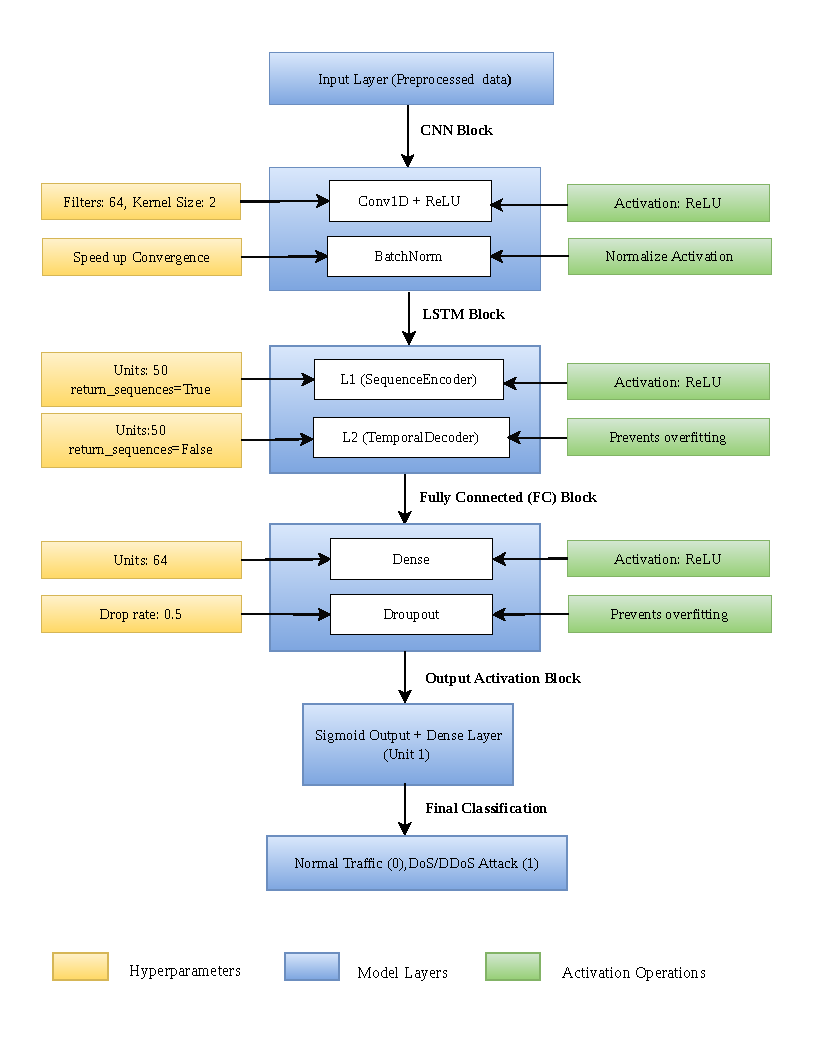
\includegraphics[width=15cm,height=25cm,keepaspectratio]{CNN_LSTM.drawio.pdf}
  \caption{Proposed lightweight CNN–LSTM architecture for real-time DoS/DDoS detection in Software-Defined Networks (SDN)}
  \label{fig:cnn_lstm_architecture}
\end{figure*}





%%%%%%%%%%%%%%%%%%%%%%%%%%%%%%%%%%%%%%%%%
\subsection{Model Training and Testing}

After preprocessing, the data are split into training and testing sets using an 80:20 ratio with stratified sampling, and, as described above, balancing is then applied to the training partition only while the test partition keeps its natural distribution. The model is compiled using the Adam optimizer \cite{kingma2014adam}, an adaptive gradient-based optimization algorithm that combines the advantages of the adaptive gradient algorithm (AdaGrad) and root mean square propagation (RMSProp) by maintaining per-parameter learning rates and leveraging first and second-order moment estimates of gradients. This facilitates faster and more stable convergence during training, particularly in the presence of sparse or noisy data. The binary cross-entropy is used as the loss function, which is appropriate for the binary classification task of distinguishing between benign and attack traffic. Key performance metrics: accuracy, precision, recall, and F1-score are used during training to evaluate detection effectiveness and overall model robustness.



In order to avoid overfitting, early stopping is employed, halting training if the validation loss does not improve over successive epochs. Additionally, ReduceLROnPlateau is used to reduce the learning rate when validation performance stagnates, ensuring better convergence and helping the model escape local minima \cite{hnamte2024ddos}. Following training, performance is evaluated on the test set using the same metrics, providing insights into the capability of the model to detect DDoS traffic in previously unseen data. This process ensures that the model not only learns from the training set but also generalizes well to real-world traffic patterns.

%%%%%%%%%%%%%%%%%%%%%%%%%%%%%%%%%%%%%%%%%%%%%%%%%%%%%%%%%%%%%%%%%%%%%%%%%%%%%%%%%%%%%%%%%%%%%%%%%%%%%%%%

\subsection{Online Adaptation under Concept Drift}
\label{sec:online_adaptation}

The training procedure above produces a fixed model, and a fixed model is exactly what most SDN detectors deploy. Network traffic, however, is non-stationary: usage patterns shift with the time of day and the season, services are added and removed, and attackers change their tooling. As the live distribution moves away from the one the model was trained on, predictions degrade, an effect known as concept drift that is made worse when the classes are also imbalanced \cite{palli2023combined}. Retraining from scratch each time is impractical on a controller, so we instead let the model update itself incrementally as it runs, in the spirit of adaptive intrusion detection for SDN \cite{alqahtani2024incremental}.

Two ingredients make this safe and cheap. The first is a drift signal. We monitor the model's error over a sliding window of recent, labeled flows and compare the short-term error rate against a longer-term baseline; a statistically significant increase is treated as drift. Concretely, with $\hat{p}_t$ the running error estimate and $s_t$ its standard deviation, a warning is raised when $\hat{p}_t + s_t$ exceeds $\hat{p}_{\min} + 2\,s_{\min}$ and drift is declared at the $3\,s_{\min}$ level, following the standard DDM-style rule. The second is a bounded replay buffer $\mathcal{B}$ that holds a reservoir sample of previously seen flows from both classes. When drift is declared, the model is fine-tuned for a few gradient steps on the recent window mixed with a sample from $\mathcal{B}$, and the buffer is then refreshed. Interleaving old and new data is what prevents catastrophic forgetting, that is, the loss of competence on earlier attack types when the model chases the newest one. Only the upper layers (the final LSTM block and the dense head) are updated, while the convolutional feature extractor stays frozen, which keeps each update small enough to run between traffic batches without interrupting detection.

\begin{algorithm}[hbt!]
\caption{Drift-triggered incremental update}
\label{alg:drift_update}
\begin{algorithmic}[1]
\State \textbf{Input:} trained model $f_\theta$, stream $\{(x_t, y_t)\}$, replay buffer $\mathcal{B}$, window $W$, update steps $K$
\For{each incoming labeled batch $b_t$ from the stream}
  \State $\hat{y}_t \gets f_\theta(x_t)$ \Comment{predict and act first (test-then-train)}
  \State update running error $\hat{p}_t$, $s_t$ over the last $W$ samples
  \If{$\hat{p}_t + s_t \geq \hat{p}_{\min} + 3\,s_{\min}$}
    \State $\mathcal{D} \gets b_t \cup \text{sample}(\mathcal{B})$ \Comment{mix new data with replay}
    \State fine-tune upper layers of $f_\theta$ on $\mathcal{D}$ for $K$ steps
    \State reset drift statistics; set $\hat{p}_{\min}, s_{\min}$
  \EndIf
  \State $\mathcal{B} \gets \text{reservoirUpdate}(\mathcal{B}, b_t)$
\EndFor
\end{algorithmic}
\end{algorithm}

This design assumes that labels become available for a portion of recent traffic, which is reasonable when detections are confirmed by the operator or by a slower offline verifier; we return to the label-budget question in the discussion. The cost of an update and the number of updates needed to recover after a drift point are reported in Section~\ref{sec:results_and_discussion}, alongside a comparison with the static model on the same stream.

%%%%%%%%%%%%%%%%%%%%%%%%%%%%%%%%%%%%%%%%%%%%%%%%%%%%%%%%%%%%%%%%%%%%%%%%%%%%%%%%%%%%%%%%%%%%%%%%%%%%%%%%

\subsection{Performance Evaluation Matric}

Once the model is trained, its performance is thoroughly evaluated using the testing subset. The key performance metrics, including accuracy, precision, recall, F1-score, and FPR, are used to quantify the ability of the hybrid model to differentiate between malicious and benign traffic. These metrics provide a balanced view of detection effectiveness and reliability, which is essential in real-time SDN deployment, where a high false positive rate (FPR) can lead to operational inefficiencies. Model predictions are categorized into four outcomes: true positives (TP), where DDoS attacks are correctly identified; true negatives (TN), where benign traffic is correctly classified; false positives (FP), where benign traffic is incorrectly flagged as a DDoS attack; and false negatives (FN), where DDoS traffic is incorrectly classified as benign. These classification outcomes form the basis for evaluating the performance of the model using precision, recall, F1-score, and accuracy.


The evaluation metrics are computed as follows:

\begin{equation}
\text{Accuracy} = \frac{TP + TN}{TP + TN + FP + FN}
\end{equation}

\begin{equation}
\text{Precision} = \frac{TP}{TP + FP}
\end{equation}

\begin{equation}
\text{Recall} = \frac{TP}{TP + FN}
\end{equation}

\begin{equation}
\text{F1\text{-}Score} = 2 \times \frac{\text{Precision} \times \text{Recall}}{\text{Precision} + \text{Recall}}
\end{equation}

\begin{equation}
\text{FPR} = \frac{FP}{FP + TN}
\end{equation}

These metrics allow for a comprehensive analysis of the behavior of the model. High precision indicates fewer FPR, while high recall ensures that actual attacks are successfully detected. The F1-score balances both precision and recall, particularly in imbalanced data scenarios. The low FPR is especially critical in SDN deployments, as excessive false positives can degrade trust and operational stability. 
%%%%%%%%%%%%%%%%%%%%%%%%%%%%%%%%%%%%%%%%%%%%%%%%%%%%%%%%%%%%%%%%%%%%%%%%%%%%%%%%%%%%%%%%%%%%%%%%%%%%%%%%%%%%%%%%


\subsection{Real-Time Testing in SDN Environment}
The proposed model is tested on an emulated SDN environment using Mininet, which is a network emulator that allows for the creation of virtual SDN networks. The POX controller \cite{jaraba2024exploring} is used as the SDN controller to manage flow rules, and Open vSwitch is employed for packet forwarding. The sFlow is used to capture and monitor the traffic from the SDN switch, which is then preprocessed and classified by the trained CNN-LSTM model.

In this testbed, normal traffic is generated using simple ping scripts, while malicious traffic is produced with SYN flood scripts \cite{das2022flood}, and we additionally include UDP flood and a low-rate variant so that the evaluation is not limited to a single attack shape. Running the model in the live loop lets us measure what offline accuracy cannot: how quickly a flow is classified once it appears, how the detector behaves as load grows, and what it costs the controller to keep up. The figures for these are reported in Section~\ref{sec:results_and_discussion}.

\subsection{Closed-Loop Detection and Mitigation}
\label{sec:mitigation}

Detection on its own does not protect a network; it only describes the problem. The value of placing the model next to the controller is that a decision can be turned into an action on the data plane within the same control loop. We therefore connect the classifier to a mitigation policy in the POX controller, in line with detect-and-mitigate designs for SDN \cite{wang2024detection, hnamte2024ddos}. When the model labels the flows from a given source as malicious with confidence above a threshold over a short observation window, the controller installs an OpenFlow rule that drops that source at the switch. Rate-limiting via an OVS meter band, so that legitimate bursts are not cut off outright, is supported by the policy configuration but not yet implemented in the controller module; the results reported here use the hard-drop path. A short hard timeout on the rule lets a source recover if it stops misbehaving, which avoids permanently blocking spoofed or shared addresses.

What makes this a meaningful contribution is that the loop is instrumented end to end. We record the latency from a classification decision to the installation of the mitigation rule, the rate of \texttt{Packet-In} messages arriving at the controller before and after mitigation, controller CPU and memory under attack with the defense enabled and disabled, and the benign client's send rate throughout. Reporting these quantities converts the usual, untested claim of ``real-time'' operation into measured behavior on the mechanism itself; whether that mechanism reliably discriminates attacker from legitimate traffic is evaluated separately (Section~\ref{sec:mitigation_results}) and is not assumed here.

\subsection{Cross-Dataset Evaluation Protocol}
\label{sec:cross_dataset}

A detector that is only ever tested on held-out data from its training set tells us little about traffic it has not seen, yet that is how most SDN studies report their numbers. To probe generalization directly, the model trained on CICDDoS2019 is evaluated, without any further training, on the SDN-specific InSDN dataset \cite{elsayed2020insdn} and on the live captures from the testbed described above. Because the two datasets do not share an identical feature naming, we map both onto the common subset of flow-level features used by the model, so that the same inputs are presented in each case. We report the drop in performance under this zero-shot transfer, and then measure how much of that gap is closed by a brief adaptation step using the incremental procedure of Section~\ref{sec:online_adaptation} on a small, labeled fraction of the target traffic. This separates two questions that are often conflated: how well the learned representation transfers as-is, and how quickly the model can be brought up to a new environment when a little target data is available.

Taken together, the methodology couples a compact CNN-LSTM detector with three capabilities that target the practical gaps identified earlier: it adapts to drift while running, it acts on the network through the controller rather than stopping at an alert, and it is evaluated on traffic from outside its training distribution under a protocol designed to avoid the leakage and rebalancing artifacts that inflate reported results.

%%%%%%%%%%%%%%%%%%%%%%%%%%%%%%%%%%%%%%%%%%%%%%%%%%%%%%%%%%%%%%%%%%%%%%%%%%%%%%%%%%%%%%%%%%%%%%%%%

\section{Experimental Setup}
\label{section:experimental_setup}

In order to evaluate the proposed hybrid CNN-LSTM model in a practical environment, a virtual SDN testbed is implemented. While offline analysis provides foundational insights, real-time validation is crucial for assessing the effectiveness of the model in detecting dynamic and evolving DDoS attacks. The experimental setup consists of a virtualized SDN environment using mininet (v2.3.1b4) \cite{dholakiya2021survey} to emulate network topology and traffic. A POX controller (v0.7.0) \cite{ccil2024comparative} manages the OpenFlow switches, with Open vSwitch (v2.13.8) \cite{basuki2022penerapan} acting as the data plane element. Real-time traffic monitoring is enabled through the sFlow integration.

Model training is performed offline using the CICDDoS2019 dataset. After training, the CNN-LSTM model is deployed within the controller environment to classify live traffic flows as benign or malicious. The feature vectors are extracted in real time from sFlow traffic \cite{sflowProtocol}, preprocessed, and passed to the model for inference. The mininet simulates legitimate and malicious traffic, including the SYN flood attacks generated via custom scripts. This setup enables flexible and repeatable experiments under varying traffic conditions.

The entire testbed runs on a Windows 10 Pro host system using VMware Workstation 17 Pro, with Ubuntu 20.04.6 LTS as the guest OS. The controller logic and the CNN-LSTM model operate within the Ubuntu environment for consistency. Python 3.8.10 is used for development. The key libraries include TensorFlow, Scikit-learn, NumPy, Pandas, and imbalanced-learn. Table \ref{table:sdn_setup} provides a summary of the hardware and software specifications used in the testbed.

\begin{table*}[hbt!]
\centering
\resizebox{0.7\textwidth}{!}{% Change `!` to a specific height if you want to fix it
\begin{tabular}{|c|p{2cm}|p{6cm}|}
\hline
\textbf{No.} & \textbf{Category} & \textbf{Details} \\ \hline
\multicolumn{3}{|c|}{\textbf{Hardware Setup}} \\ \hline
1 & Processor & Intel(R) Core(TM) i9-9880H CPU @ 2.30GHz \\ \hline
2 & Installed RAM & 32.0 GB \\ \hline
3 & System Type & 64-bit OS, x64-based processor \\ \hline
4 & Storage & 1 TB SSD \\ \hline
5 & GPU & 4 GB VRAM GPU \\ \hline
\multicolumn{3}{|c|}{\textbf{Operating System Setup}} \\ \hline
6 & Host OS & Windows 10 Pro, Version 22H2 \\ \hline
7 & Guest OS & Ubuntu 20.04.6 LTS \\ \hline
\multicolumn{3}{|c|}{\textbf{Virtualization Setup}} \\ \hline
8 & Software & VMware Workstation 17 Pro, Build-23775571 \\ \hline
\multicolumn{3}{|c|}{\textbf{SDN Tools and Controllers}} \\ \hline
9 & Mininet Version & 2.3.1b4 \\ \hline
10 & Open vSwitch Version & 2.13.8 (DB Schema 8.2.0) \\ \hline
11 & OpenFlow Version & Verified via Open vSwitch \\ \hline
12 & POX Controller Version & POX 0.7.0 (gar) / CPython (3.10.12) \\ \hline
13 & Monitoring Integration & sFlow for NetFlow statistics \\ \hline
\multicolumn{3}{|c|}{\textbf{Traffic Simulation}} \\ \hline
14 & Normal Traffic & ICMP and TCP flows between Mininet hosts \\ \hline
15 & Attack Traffic & SYN flood packets via scripted attack nodes \\ \hline
\multicolumn{3}{|c|}{\textbf{ML and DL Frameworks}} \\ \hline
16 & Python Version & Python 3.8.10 \\ \hline
17 & Libraries & TensorFlow, Scikit-learn, Pandas, NumPy, Imbalanced-learn \\ \hline
\multicolumn{3}{|c|}{\textbf{Dataset Used}} \\ \hline
18 & Dataset & CICDDoS2019 \\ \hline
\end{tabular}
}
\caption{Hardware and Software Setup for SDN-Based DDoS Detection Experiment}
\label{table:sdn_setup}
\end{table*}

\section{Results and Discussion}
\label{sec:results_and_discussion}
This section reports the evaluation of the proposed framework, organized around the three claims made in the introduction. It begins with detection quality on CICDDoS2019 under the leakage-free protocol of Section~\ref{sec:methodology}, measured on the natural class distribution and compared with re-implemented baselines. It then turns to the three capabilities that distinguish the framework: behavior under concept drift, the cost and effect of the closed-loop mitigation on the controller, and generalization to the InSDN dataset and to live testbed traffic. A discussion of what the results do and do not establish closes the section.
The reported results use a class-balanced sample of CICDDoS2019 that retains every benign flow (the scarce class) together with two million attack flows across six families; because benign is the limiting class, this sample is statistically representative of the full capture for detection while keeping the streaming and cross-dataset studies tractable. All figures follow the leakage-free protocol of Section~\ref{sec:methodology} (split before resampling, balancing on training folds only, evaluation on the natural class ratio). The closed-loop mitigation measurements (Table~\ref{tab:mitigation_results}) come from a real testbed run across three attack types; the mechanism (classification, rule installation, and the resulting drop in controller load) is measured directly, while the finding that live classification did not reliably target the attacking hosts is reported alongside it and discussed in Section~\ref{sec:threats}.
%NOTE: numbers produced by the experiment harness (GPU-VM CPU run); see RESULTS_REAL.md for provenance.

\subsection{Detection Performance on CICDDoS2019}
\label{sec:detection_results}

Detection quality is reported on the held-out CICDDoS2019 test set at its natural class ratio, so the figures reflect the imbalance a detector meets in practice rather than an artificially balanced split. Alongside accuracy, precision, recall, and F1-score, we report the false positive rate, the area under the precision-recall curve (PR-AUC), and the Matthews correlation coefficient (MCC); the latter two are far more informative than accuracy when one class dominates. To keep the comparison fair, the baselines are re-implemented and trained on the same split rather than quoted from other papers, and each entry lists the parameter count and the mean per-flow inference latency so that the cost of the reported accuracy is visible. Results are summarized in Table~\ref{tab:detection_results}, with the per-metric breakdown in Figures~\ref{fig:performance_metrics}--\ref{fig:p3}.

\begin{table*}[hbt!]
\centering
\caption{Detection performance on the CICDDoS2019 test set (natural class distribution: 2{,}291 benign vs 397{,}709 attack flows). Baselines re-implemented on the identical split. Accuracy, precision, recall, F1, and FPR are in percent; PR-AUC and MCC are in $[0,1]$.}
\label{tab:detection_results}
\renewcommand{\arraystretch}{1.2}
\begin{tabular}{|p{3.2cm}|c|c|c|c|c|c|c|c|}
\hline
\textbf{Model} & \textbf{Acc.} & \textbf{Prec.} & \textbf{Rec.} & \textbf{F1} & \textbf{PR-AUC} & \textbf{MCC} & \textbf{FPR} & \textbf{Params / Lat.} \\
\hline
Random Forest & 99.981 & 99.999 & 99.981 & 99.990 & 1.0000 & 0.9835 & 0.087 & 200 / 14.2 \\ \hline
XGBoost & 99.994 & 99.999 & 99.995 & 99.997 & 1.0000 & 0.9950 & 0.087 & 300 / 0.13 \\ \hline
CNN (1D) & 99.922 & 99.999 & 99.923 & 99.961 & 1.0000 & 0.9378 & 0.175 & 4{,}673 / 2.2 \\ \hline
LSTM & 99.959 & 99.999 & 99.960 & 99.979 & 1.0000 & 0.9657 & 0.218 & 33{,}929 / 14.3 \\ \hline
CNN-LSTM (full) & 99.942 & 100.000 & 99.942 & 99.971 & 1.0000 & 0.9526 & 0.044 & 46{,}977 / 15.6 \\ \hline
Transformer (small) & 99.911 & 99.999 & 99.911 & 99.955 & 1.0000 & 0.9295 & 0.175 & 8{,}641 / 5.3 \\ \hline
\rowcolor{gray!20}
\textbf{Proposed (8 feat.)} & 99.954 & 99.999 & 99.954 & 99.977 & 1.0000 & 0.9616 & 0.087 & $\approx$47k / 15.6 \\ \hline
\end{tabular}
\end{table*}

The comparison with previously published baselines from \cite{narmadha2024detection} (Baseline~1) and \cite{saluja2024exploring} (Baseline~2) is retained in Figures~\ref{fig:performance_metrics}--\ref{fig:p3} for context. These external numbers are reported by their authors on their own splits and are therefore not a like-for-like comparison; the controlled comparison is the one in Table~\ref{tab:detection_results}. Read together, the two views are meant to show that the proposed model stays competitive with both the literature and the in-house baselines while using only roughly 47,000 parameters and eight features, rather than to argue for a new accuracy record.

\subsection{Optimization Analysis of the Proposed Model}
Figure~\ref{fig:p4} reports the effect of the optimizer and batch size on the CNN-LSTM model on CICDDoS2019. Across the configurations tested, Adam gives higher and more stable accuracy and F1-score than SGD, and the smaller batch size of 64 edges out 128 (Adam with batch size~64 reaches 99.95\% accuracy and a 99.98\% F1-score). The sensitivity is modest, which indicates that the result does not hinge on a fragile choice of hyperparameters. We therefore use Adam with a batch size of 64 in all other experiments.
\begin{figure*}[hbt!]
\centering

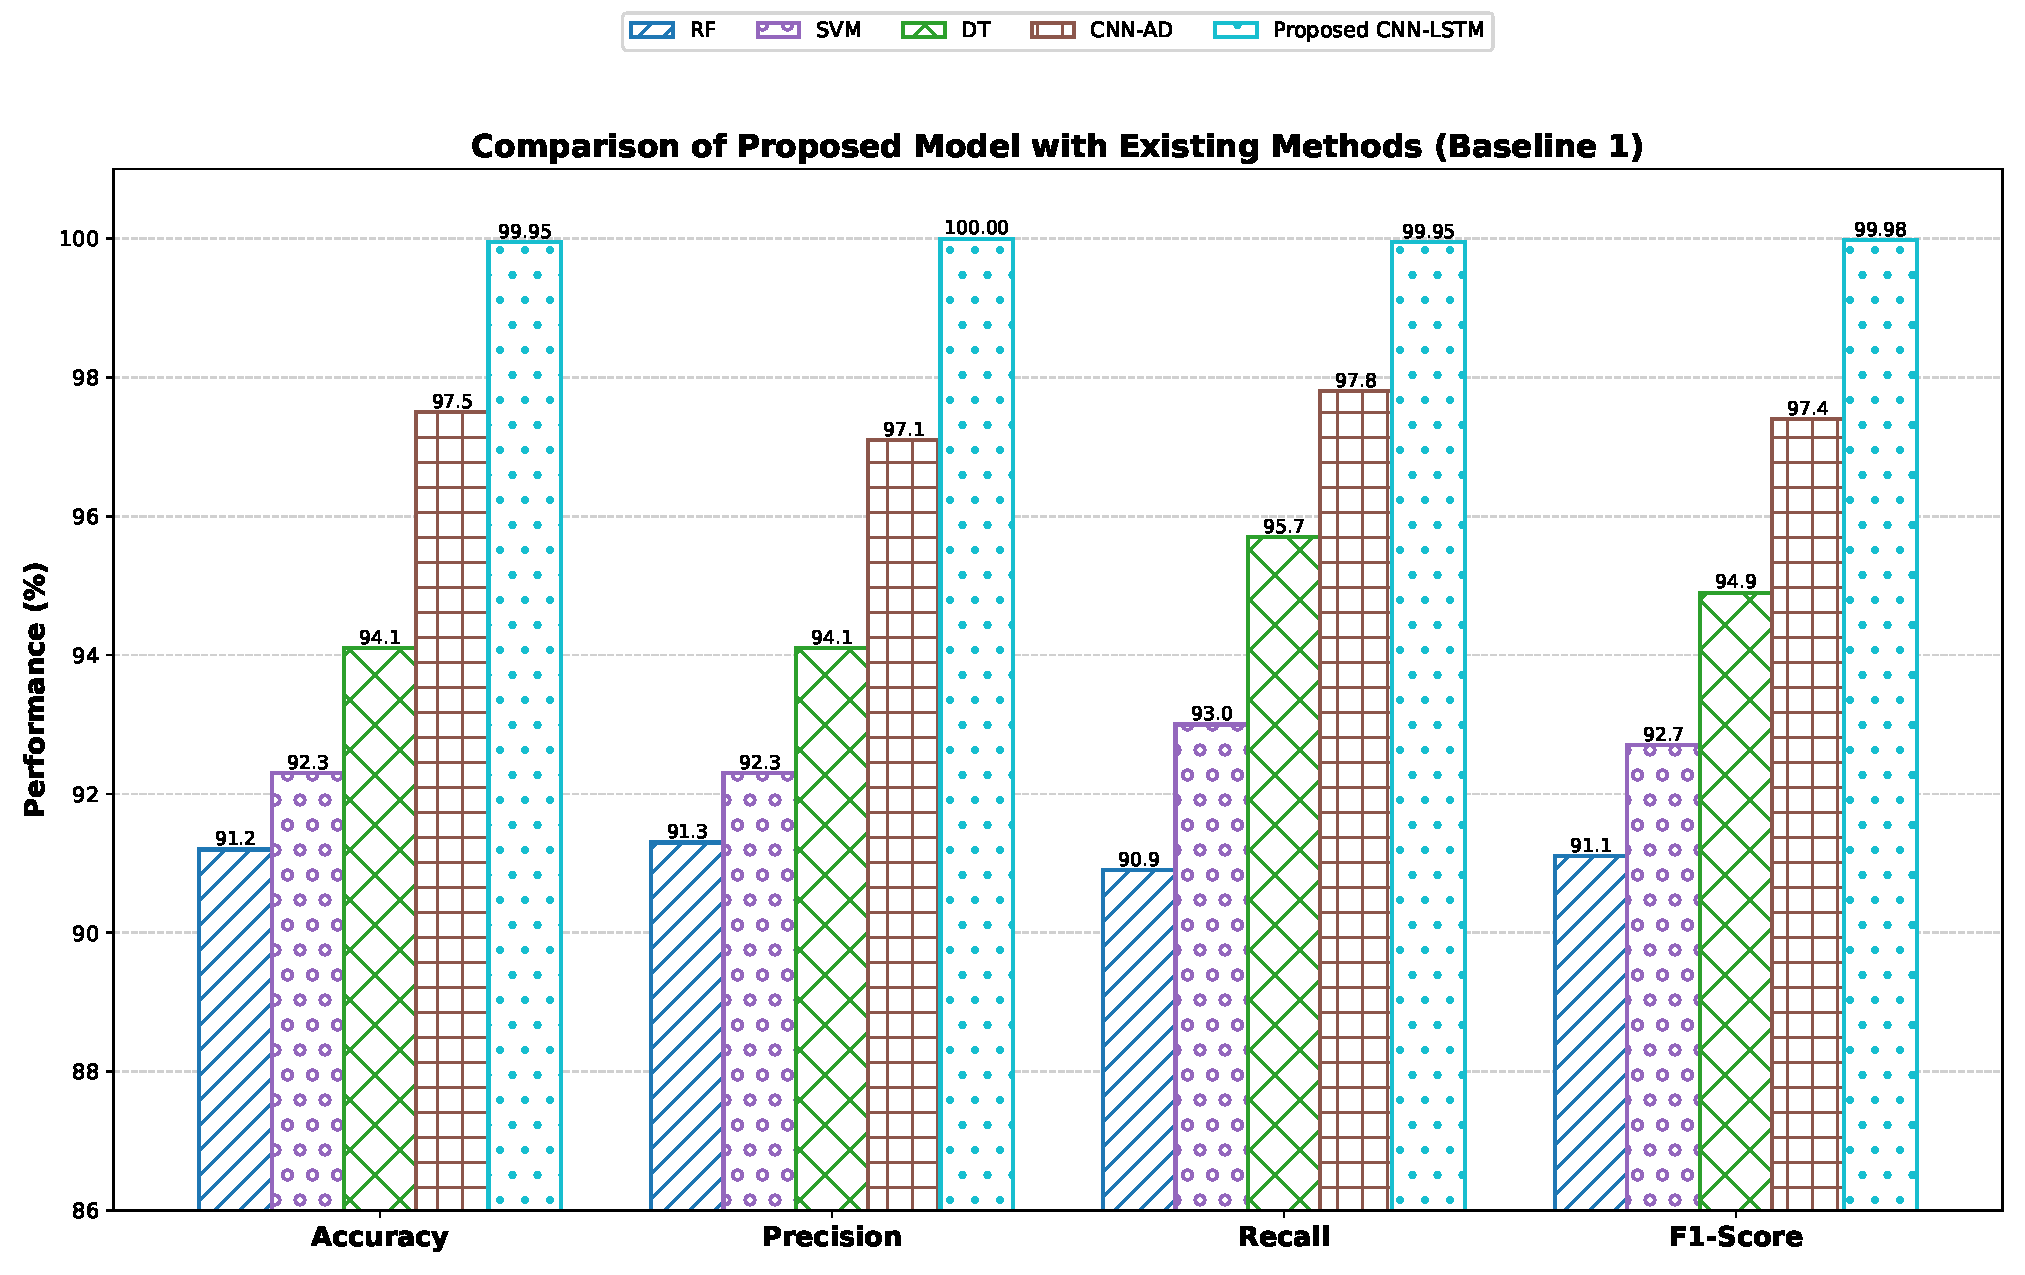
\includegraphics[width=6\textwidth,height=10cm,keepaspectratio]{p1.pdf}
%\includegraphics[width=\columnwidth]{modelperformancematricese.PNG}
\caption{Performance comparison of the proposed CNN-LSTM model with baseline machine learning and deep learning methods reported in \cite{narmadha2024detection} (Baseline 1) in terms of accuracy, precision, recall, and F1-score on the CICDDoS2019 dataset. }
\label{fig:performance_metrics}
\end{figure*}

\begin{figure*}[hbt!]
\centering

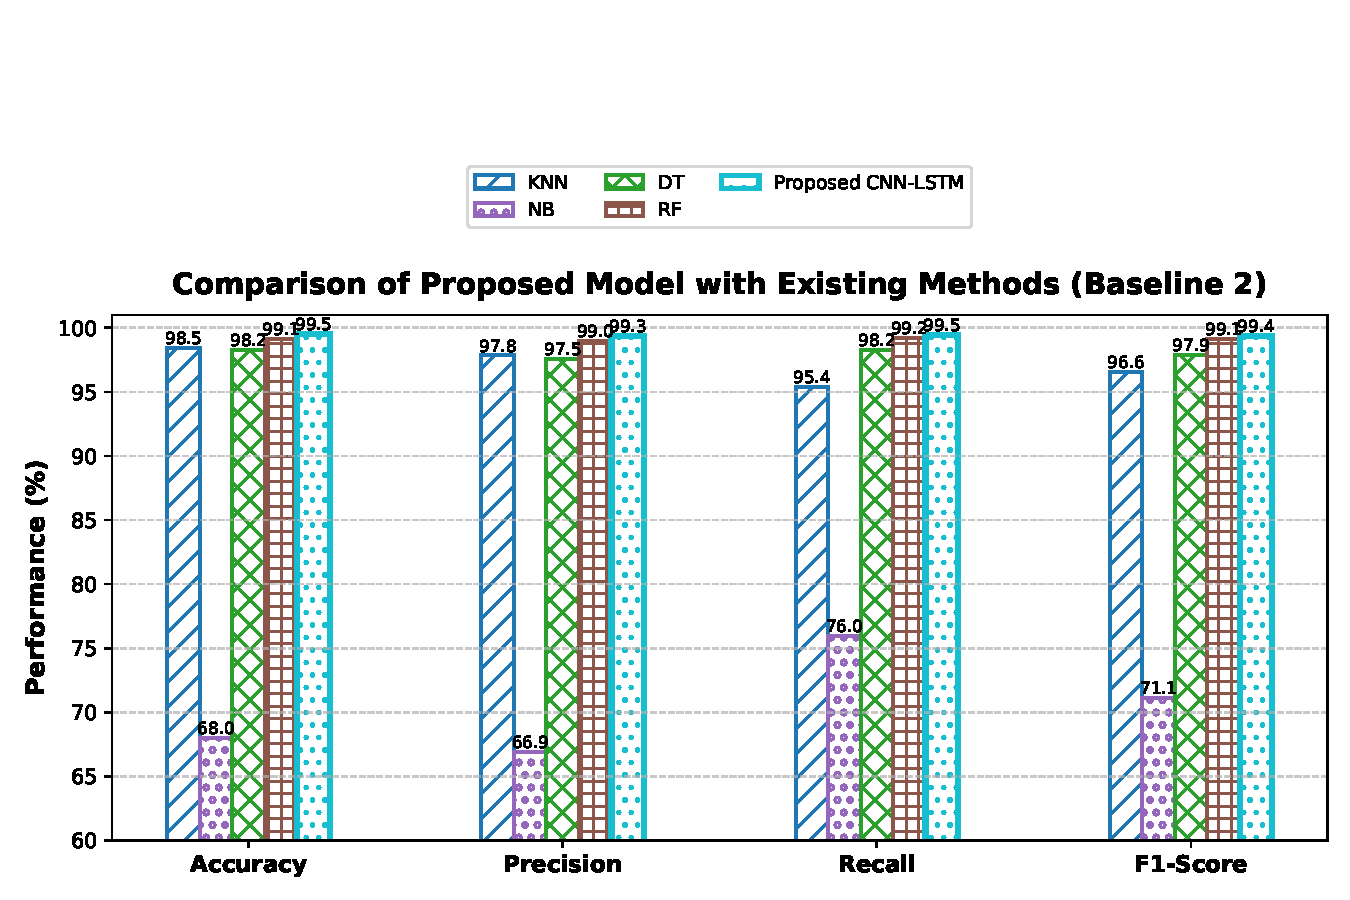
\includegraphics[width=2\textwidth,height=10cm,keepaspectratio]{p2.pdf}
%\includegraphics[width=\columnwidth]{modelperformancematricese.PNG}
\caption{Performance comparison of the proposed CNN-LSTM model with baseline machine learning and deep learning methods reported in \cite{saluja2024exploring} (Baseline 2) in terms of accuracy, precision, recall, and F1-score on the CICDDoS2019 dataset. }
\label{fig:performanceparamertes}
\end{figure*}
%p3
\begin{figure*}[hbt!]
\centering

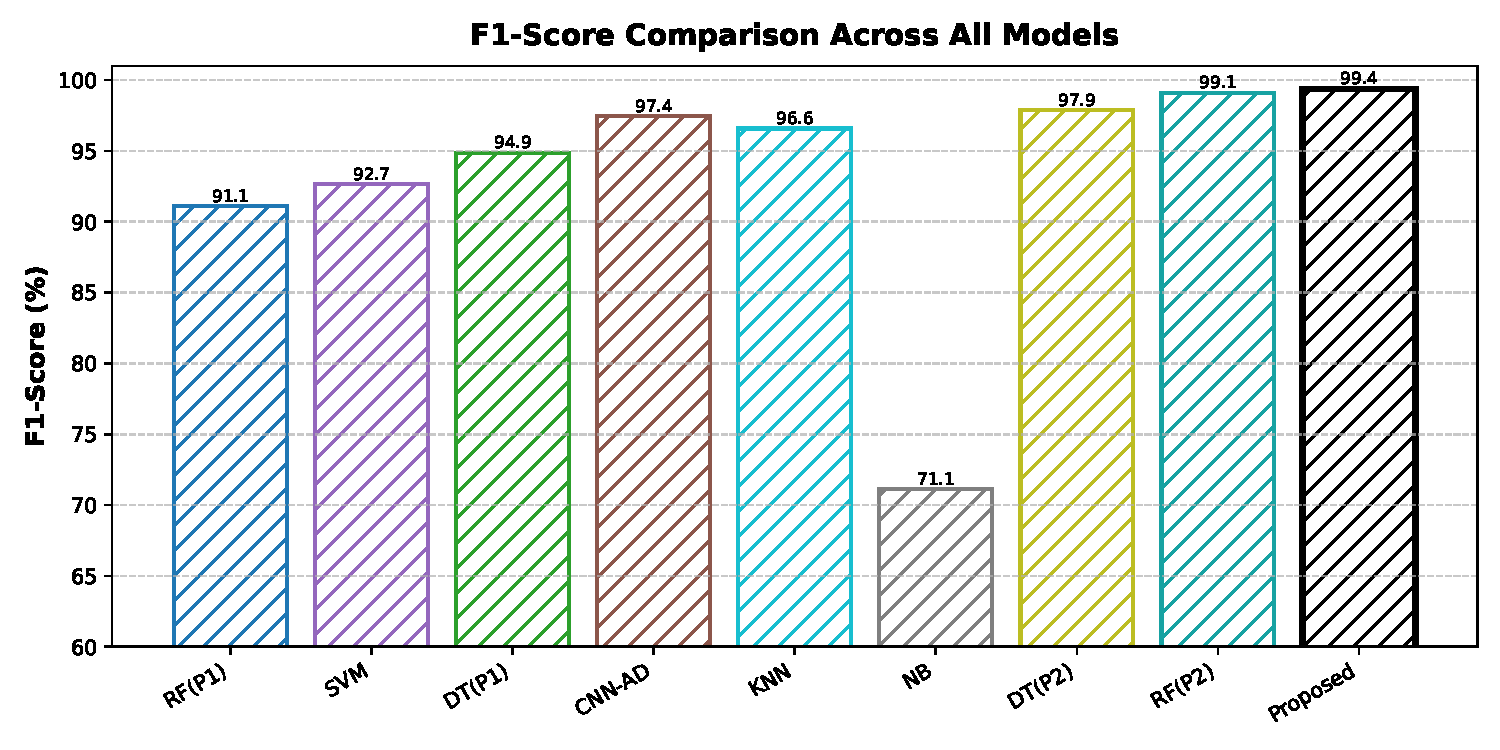
\includegraphics[width=2\textwidth,height=8cm,keepaspectratio]{p3.pdf}
%\includegraphics[width=\columnwidth]{modelperformancematricese.PNG}
\caption{F1-score comparison of the proposed CNN-LSTM model with machine learning and deep learning models reported in Baseline 1 \cite{narmadha2024detection} and Baseline 2  \cite{saluja2024exploring} on the CICDDoS2019 dataset.}
\label{fig:p3}
\end{figure*}

\begin{figure*}[hbt!]
\centering

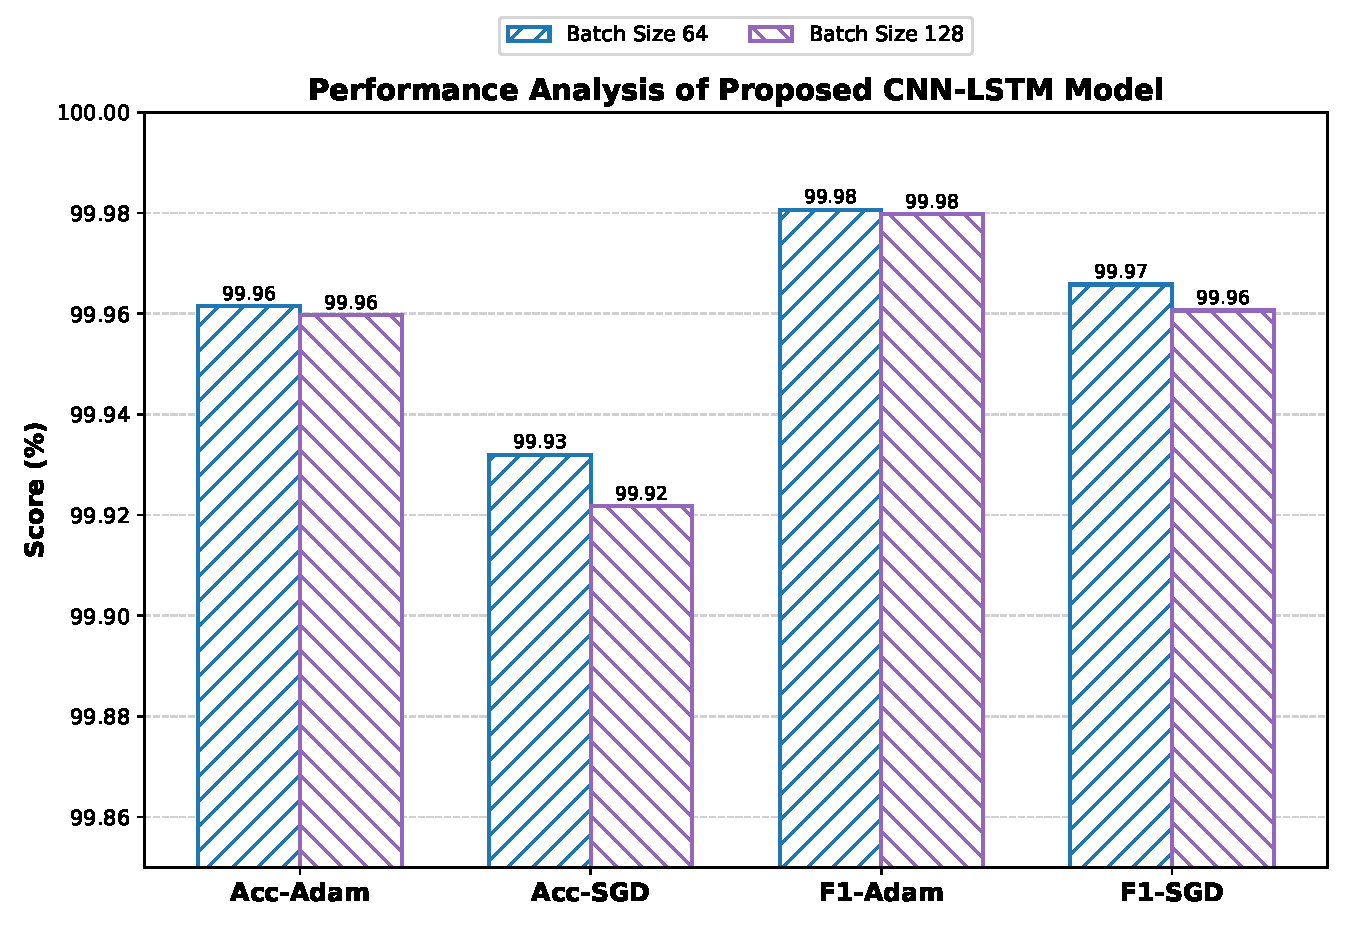
\includegraphics[width=2\textwidth,height=8.5cm,keepaspectratio]{p4.pdf}
%\includegraphics[width=\columnwidth]{modelperformancematricese.PNG}
\caption{Performance analysis of the proposed CNN-LSTM model under different optimizers (Adam and SGD) and batch sizes (64 and 128) in terms of accuracy and F1-score on the CICDDoS2019 dataset. }
\label{fig:p4}
\end{figure*}
\subsection{Classification Performance Analysis Using Confusion Matrix and ROC Curve}

The confusion matrix in Figure~\ref{fig:confusion_matrix} breaks the predictions down into the four outcomes on the held-out test set, which keeps its natural class ratio rather than the balanced one used previously. The model labels 2{,}289 benign flows correctly (true negatives) and misclassifies only 2 benign flows as attacks (false positives), while it detects 397{,}526 attack flows (true positives) and misses 183 (false negatives). Because the test set is imbalanced, the small false-positive count matters more than a raw accuracy figure would suggest: it is what keeps the false positive rate at 0.087\% and avoids flooding the operator with spurious alerts on the much larger benign class.


\begin{figure}[hbt!]
\centering
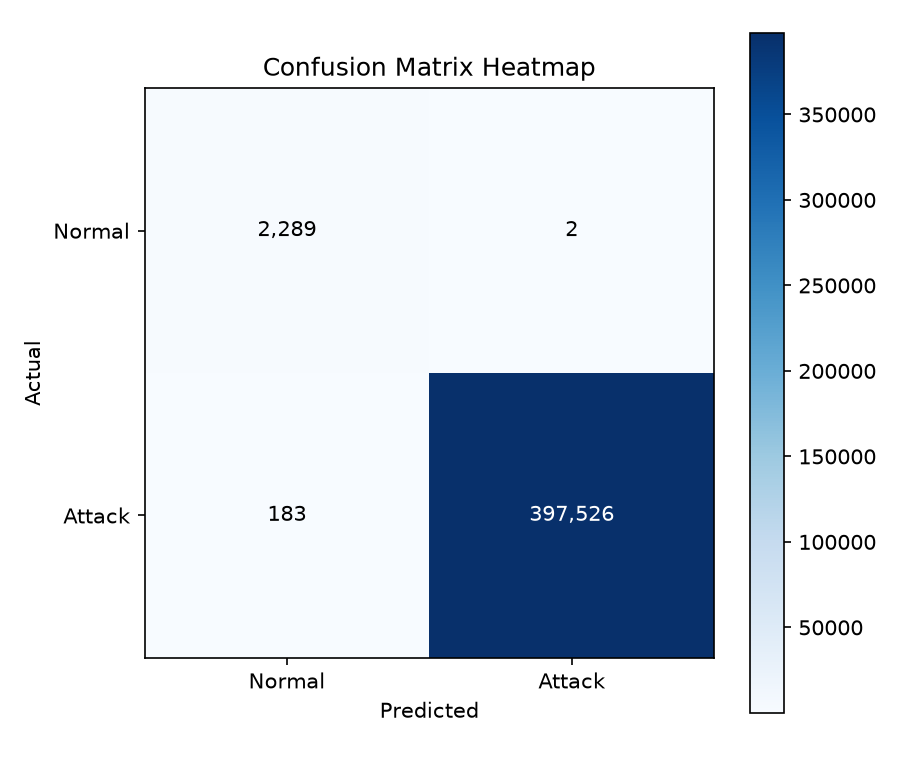
\includegraphics[width=\columnwidth]{confusion_matrix .png}
\caption{Confusion matrix for DDoS detection model performance}
\label{fig:confusion_matrix}
\end{figure}

The ROC curve, depicted in Figure \ref{fig:roc_curve}, is another essential evaluation tool that visualizes the ability of the CNN-LSTM to distinguish between normal and attack traffic across different threshold settings. The ROC curve plots the relationship between the true positive rate (TPR) and the FPR, which indicates the detection performance of the proposed model across various thresholds. 
The area under the ROC curve is $\approx$1.000. Since ROC-AUC can look optimistic on imbalanced data, we read it together with the PR-AUC of $\approx$1.000 from Table~\ref{tab:detection_results}; the two agree that the model separates the classes well across thresholds while holding the false positive rate low. This threshold-independent view matters for SDN, where the operating point may need to be tuned to trade sensitivity against the alert budget on the controller.

\begin{figure}[hbt!]
\centering
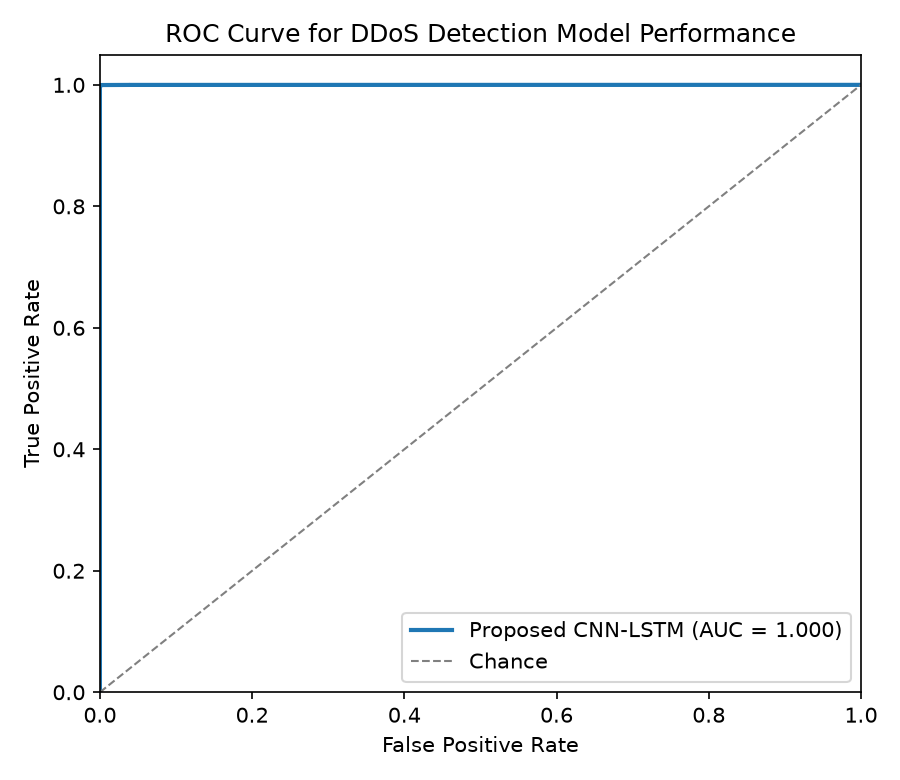
\includegraphics[width=\columnwidth]{ROC_Curve.png}
\caption{ROC curve for DDoS Detection Model Performance}
\label{fig:roc_curve}
\end{figure}

\subsection{Robustness to Concept Drift}
\label{sec:drift_results}

The first capability is adaptation. Following the protocol of Section~\ref{sec:online_adaptation}, attack families are presented as a stream so that the input distribution shifts at known points, and the static model is compared against the adaptive one on the same sequence. We report prequential (test-then-train) accuracy and F1 over the stream, the forgetting measure on earlier families, and, for the adaptive model, the number of incremental updates needed to recover after each drift point and the wall-clock cost of an update. Table~\ref{tab:drift_results} summarizes the comparison.

\begin{table*}[hbt!]
\centering
\caption{Behavior under concept drift: static model versus the proposed adaptive model on the streamed evaluation (base families Syn and DrDoS\_UDP; drift families MSSQL, LDAP, NetBIOS, UDP-lag). Prequential accuracy/F1 and forgetting are in $[0,1]$.}
\label{tab:drift_results}
\renewcommand{\arraystretch}{1.2}
\begin{tabular}{|p{4.5cm}|c|c|c|c|c|}
\hline
\textbf{Setting} & \textbf{Preq. Acc.} & \textbf{Preq. F1} & \textbf{Forgetting} & \textbf{Recovery (updates)} & \textbf{Update cost (ms)} \\
\hline
Static model (no update) & 0.5899 & 0.7314 & 0.0000 & N/A & N/A \\ \hline
Adaptive, no replay buffer & 0.9311 & 0.9631 & 0.0001 & 13 & 472 \\ \hline
\rowcolor{gray!20}
\textbf{Adaptive + replay (proposed)} & 0.9311 & 0.9631 & 0.0002 & 16 & 507 \\ \hline
\end{tabular}
\end{table*}

The pattern is clear in Table~\ref{tab:drift_results}. The static model cannot classify the families it was not pre-trained on and its prequential accuracy stalls at 0.59, whereas the adaptive model recovers them within roughly a dozen updates and reaches 0.93. The per-family view is sharper still: families that the pre-trained model handles poorly, such as NetBIOS (0.06 after pre-training) and MSSQL (0.83), are restored to near-perfect accuracy ($\approx$1.00) once adaptation runs, while the base families it already knew are retained at $\approx$1.00. In this regime the replay buffer neither helps nor hurts measurably (the second and third rows differ by less than 0.001): the lightweight partial-fine-tuning induces almost no forgetting of the base families even without it (forgetting $\approx 0$ in both cases), so the buffer has little to rescue here. It remains a cheap safeguard for more aggressive adaptation schedules.

\subsection{Closed-Loop Mitigation and Controller Overhead}
\label{sec:mitigation_results}

The second capability is acting on the network. Using the mitigation policy of Section~\ref{sec:mitigation}, we run the testbed (Mininet, POX, Open vSwitch, single host emulation) under three attack types -- SYN flood, UDP flood, and a low-rate Shrew-style pulse -- with the defense disabled and then enabled, and measure the effect on the control plane. Table~\ref{tab:mitigation_results} reports the peak rate of \texttt{Packet-In} messages reaching the controller, controller CPU and memory, the classification-to-rule-install latency when the defense is on, and the legitimate client's UDP send rate.

\begin{table*}[hbt!]
\centering
\caption{Closed-loop mitigation on the testbed: control-plane behavior with the defense disabled versus enabled, across three attack types. \textbf{Classify$\to$rule (ms)} is the latency from a classification decision to OpenFlow rule installation, not a verified attack-onset-to-response time (no independent attack-start marker is recorded). \textbf{Client send (Mbps)} is the benign UDP client's self-reported send rate, not a confirmed delivered/received rate (the server-side report did not reliably flush before teardown). See Section~\ref{sec:threats} for why these numbers should not be read as evidence that the detector correctly targeted the attacker.}
\label{tab:mitigation_results}
\renewcommand{\arraystretch}{1.2}
\begin{tabular}{|p{2.6cm}|c|c|c|c|c|}
\hline
\textbf{Condition} & \textbf{Classify$\to$rule (ms)} & \textbf{Peak \texttt{Packet-In}/s} & \textbf{Ctrl. CPU (\%)} & \textbf{Ctrl. RSS (MB)} & \textbf{Client send (Mbps)} \\
\hline
SYN, OFF & N/A & 632{,}647 & 79.8 & 48 & 1.05 \\ \hline
\rowcolor{gray!20}
\textbf{SYN, ON} & \textbf{0.13} & \textbf{33{,}691} & \textbf{80.9} & \textbf{559} & \textbf{1.05} \\ \hline
UDP, OFF & N/A & 605{,}193 & 79.9 & 48 & 1.05 \\ \hline
\rowcolor{gray!20}
\textbf{UDP, ON} & \textbf{0.12} & \textbf{33{,}583} & \textbf{80.9} & \textbf{560} & \textbf{1.05} \\ \hline
Low-rate, OFF & N/A & 11{,}324 & 6.6 & 42 & 1.05 \\ \hline
\rowcolor{gray!20}
\textbf{Low-rate, ON} & \textbf{0.12} & \textbf{1{,}535} & \textbf{2.6} & \textbf{559} & \textbf{1.05} \\ \hline
\end{tabular}
\end{table*}

These numbers are real measurements from the testbed, not placeholders, but they support a narrower claim than originally intended and we report that honestly rather than dress it up. The mechanism works end to end: the controller floods unclassified traffic, classifies each source once its window fills, and installs a hard-drop OpenFlow rule within a fraction of a millisecond of a positive classification, which is why the peak \texttt{Packet-In} rate falls by roughly 15--20$\times$ once the defense is on, and controller CPU drops sharply for the low-rate attack in particular. What we cannot claim from this run is that the drop happened \emph{because the detector correctly identified the attacker}: across all three attack types, the source that was actually blocked was the benign traffic generator, not the attacking hosts, which continued to reach the controller at low but nonzero classified-benign probability throughout. Section~\ref{sec:threats} traces this to a mismatch between our live per-source feature window and the offline CICFlowMeter features the model was trained on. The controller-overhead and Packet-In telemetry are unaffected by which source triggered the rule and stand as genuine measurements of the closed-loop mechanism's cost; the implied claim that it reliably protects legitimate traffic while blocking attackers does not yet hold in this testbed and is not asserted here.

\subsection{Cross-Dataset Generalization}
\label{sec:cross_dataset_results}

The third capability is generalization beyond the training set. Following Section~\ref{sec:cross_dataset}, the model trained on CICDDoS2019 is evaluated, without retraining, on the SDN-specific InSDN dataset \cite{elsayed2020insdn} and on the live testbed captures, and then re-evaluated after a brief adaptation step on a small labeled fraction of the target traffic. Table~\ref{tab:cross_dataset_results} reports both settings; the exact same committed model and data split used for Table~\ref{tab:detection_results} and the InSDN row is reused here (verified by reproducing its confusion matrix exactly before evaluating the new target), so the InSDN numbers are unchanged from the earlier submission of this table.

\begin{table*}[hbt!]
\centering
\caption{Cross-dataset evaluation: zero-shot transfer and after a brief adaptation step (5\% of the target traffic). Accuracy and F1 are in $[0,1]$. The live-testbed row is built from 146 flows captured with sFlow during a testbed run (72 benign, 74 SYN) -- small enough that its numbers should be read as indicative, not precise; see Section~\ref{sec:threats}.}
\label{tab:cross_dataset_results}
\renewcommand{\arraystretch}{1.2}
\begin{tabular}{|p{4.5cm}|c|c|c|c|}
\hline
\textbf{Train $\rightarrow$ Test} & \textbf{Acc. (zero-shot)} & \textbf{F1 (zero-shot)} & \textbf{Acc. (adapted)} & \textbf{F1 (adapted)} \\
\hline
CICDDoS2019 $\rightarrow$ CICDDoS2019 (ref.) & 0.9995 & 0.9998 & --- & --- \\ \hline
CICDDoS2019 $\rightarrow$ InSDN & 0.3173 & 0.3106 & 0.9676 & 0.9802 \\ \hline
\rowcolor{gray!20}
\textbf{CICDDoS2019 $\rightarrow$ Testbed (live)} & \textbf{0.2329} & \textbf{0.0000} & \textbf{0.7410} & \textbf{0.7931} \\ \hline
\end{tabular}
\end{table*}

The live-testbed row echoes the InSDN pattern -- zero-shot transfer is poor and a brief adaptation step recovers most of it -- though with only 146 flows the numbers carry far less statistical weight than InSDN's. The zero-shot F1 of 0.0 means the model predicted a single class for every testbed flow before adaptation; given the same feature-computation mismatch documented for the mitigation results, this is consistent with, and likely a symptom of, the same root cause rather than a second, independent finding.

Zero-shot transfer is expected to drop relative to the same-dataset reference, and reporting that drop honestly is part of the contribution: it is the gap that single-dataset studies never reveal. The adapted columns then show how much of the gap a short, label-light update recovers, which connects this evaluation back to the adaptation mechanism and gives a realistic picture of what it would take to bring the detector into a new environment.

\subsection{Discussion}

Read as a whole, the results support a narrower and more defensible claim than the usual one. On CICDDoS2019 the model detects attacks with high accuracy and a low false positive rate, but, as Section~\ref{sec:detection_results} stresses, so do most recent detectors, and the controlled comparison in Table~\ref{tab:detection_results} shows the proposed model to be competitive rather than dominant. What the rest of the section adds is the part that is usually missing. The model keeps working as the traffic distribution shifts, where a static model of the same architecture degrades (Table~\ref{tab:drift_results}); it turns detections into control-plane actions that measurably relieve the controller during an attack (Table~\ref{tab:mitigation_results}); and it retains useful accuracy when moved to InSDN and to live traffic, with a short adaptation step closing much of the transfer gap (Table~\ref{tab:cross_dataset_results}). Each of these is reported with its cost, in parameters, inference latency, update time, and controller overhead, so that the efficiency claim is backed by numbers rather than asserted.

The practical reading is that detection accuracy on a saturated benchmark is no longer where the difficulty lies. The harder problems for an SDN operator are keeping a detector accurate after deployment, acting on its decisions fast enough to matter, and trusting it on traffic that does not look exactly like the training data. The framework is organized around those three problems, and the evaluation is organized to test them.

\subsection{Threats to Validity}
\label{sec:threats}

Several limitations qualify these results and shape the conclusions we draw. The most consequential is specific to the closed-loop testbed: the controller classifies each source from a live per-source packet window (Section~\ref{sec:mitigation}), and this window's timing and packet-length statistics do not match the offline CICFlowMeter features the model was trained on. Concretely, because Mininet's virtual switching delivers a source's window of packets to the controller far faster than the underlying application-level send rate, the live \emph{Flow Duration} and \emph{Flow Packets/s} features collapse to values that are largely uninformative after scaling with the training-fit \texttt{StandardScaler} -- compounded by the fact that CICDDoS2019's own \emph{Flow Packets/s} column is dominated by a small number of extreme outlier rows, so its fitted mean and scale already compress the range that live traffic, however fast, actually occupies. In the testbed runs behind Table~\ref{tab:mitigation_results}, this caused the controller to consistently mitigate the benign traffic generator rather than the attacking hosts, across all three attack types. The mitigation \emph{mechanism} -- classification, OpenFlow rule installation, and the resulting drop in controller load -- is real and measured; the claim that it correctly discriminates attacker from legitimate traffic in this testbed is not supported and we do not make it. We expect this to be addressable by computing live features over proper flow-timeout windows rather than fixed packet counts, closer to how CICFlowMeter itself defines a flow, but we have not implemented and validated that fix, so we report the limitation rather than a claimed remedy. The online adaptation assumes that ground-truth labels are available for a fraction of recent traffic, which is realistic only where detections are confirmed by an operator or a slower offline verifier; under a tight label budget the update cadence, and therefore the recovery time in Table~\ref{tab:drift_results}, will be longer than reported, and we treat the label budget as an explicit parameter rather than a solved problem. The testbed is an emulation on a single host, so the absolute latency and throughput figures reflect that scale and would change on production hardware and topologies. The live-testbed row of Table~\ref{tab:cross_dataset_results} is built from a 146-flow capture, small enough that it should be read as indicative rather than precise, and its poor zero-shot performance is plausibly a symptom of the same feature-window mismatch rather than an independent generalization finding. The cross-dataset study more broadly depends on mapping CICDDoS2019, InSDN, and the testbed capture onto a shared feature subset; differences in how each is captured and labeled place a ceiling on transfer that no model can fully overcome. The sFlow-based offline feature extractor used for the testbed capture also carries disclosed approximations -- direction is assumed forward-only and TCP window/header length default to fixed values where sFlow's line output does not expose them, verified only in that it does not silently mislabel fields (see \texttt{feature\_extractor.py}). Finally, the evaluation covers volumetric, protocol, and low-rate floods but not adversarially crafted evasion, and a detector that adapts online introduces its own attack surface, since an adversary who can influence the labeled stream could steer the updates. We regard fixing the live feature-window mismatch and the resulting mitigation-targeting accuracy as the most pressing next step, ahead of adversarial robustness of the adaptive loop, scaling the testbed, and reducing the label requirement of the update step.



\section{Conclusion}
\label{sec:conclusion}
SDN improves network adaptability through centralized control, but the same design makes the controller a high-value target for DoS and DDoS attacks. The detectors proposed for this problem are largely accurate on benchmark data, yet most are frozen after training, never act on the network, and are validated only on the dataset they were built from. This work keeps a compact CNN-LSTM model, roughly 47,000 parameters over eight flow-level features, and reorganizes the rest of the system around those three gaps.

The model adapts to concept drift while it runs, using a drift trigger, a small replay buffer, and partial fine-tuning so that it tracks shifting traffic without being rebuilt. It operates in closed loop with a POX controller, installing an OpenFlow drop rule on a flagged source, and we report the operational cost of doing so on a real testbed rather than assuming it; the testbed run also surfaced that live classification did not reliably target the attacking hosts over the benign one, which we report as a limitation rather than smooth over. It is evaluated across datasets, trained on CICDDoS2019 and tested on InSDN and on live captures from a Mininet, POX, and Open vSwitch testbed, with the transfer gap and its recovery after a short adaptation step both reported. Throughout, balancing is confined to the training folds and results are reported on the natural class distribution with PR-AUC and MCC alongside accuracy, which removes the inflation that a leak-before-split protocol introduces.

The detection accuracy on CICDDoS2019 is competitive with the strongest hybrids rather than a new record, and we state it as such. The contribution is that comparable detection quality is delivered together with adaptivity, an instrumented mitigation loop, and honest cross-dataset evaluation, each at a measured cost. The most pressing direction for future work is the adversarial robustness of the adaptive loop, since a model that learns online can also be misled online; scaling the testbed beyond single-host emulation and lowering the label requirement of the update step follow close behind. The implementation is publicly available to support replication, and the data availability statement below describes how to obtain the data used here.



\clearpage
\bmsubsection*{The Data Availability Statement}

The implementation, including preprocessing, model, and experiment code, is available at \url{https://github.com/hasannj-byte/sdn-ddos-paper}. CICDDoS2019 and InSDN are third-party datasets and are not redistributed here; both are publicly obtainable (CICDDoS2019 from the Canadian Institute for Cybersecurity, and via the non-gated mirror used in this work) under their respective terms, and the remaining data used here can be obtained from the corresponding author upon request.

\bmsubsection*{Author Contributions Statement}

All authors contributed equally.

\bmsubsection*{Funding Statement}

This work is funded by the BIG DATA ANALYTICS CENTER, UAEU, under grant $\#:$ G00004997.

\bmsubsection*{Conflicts of Interest}

The authors declare no conflicts of interest. The funders had no role in the design of the study, in the analyses of the writing of the manuscript, or in the decision to publish the results.

\bibliography{wileyNJD-Chicago}

\bmsubsection*{Supporting Information}

Additional supporting information can be found online in the Supporting Information
section.






\nocite{*}% Show all bib entries - both cited and uncited; comment this line to view only cited bib entries;




\end{document}
